\documentclass{article}
\usepackage[preprint]{neurips_2026}

\usepackage[utf8]{inputenc}
\usepackage[T1]{fontenc}
\usepackage{hyperref}
\usepackage{url}
\usepackage{booktabs}
\usepackage{amsfonts}
\usepackage{amsmath}
\usepackage{amssymb}
\usepackage{amsthm}
\usepackage{microtype}
\usepackage{xcolor}
\usepackage{graphicx}

\makeatletter
\renewcommand{\@noticestring}{Extended version of the ES 678 course project. Preprint.}
\makeatother
\graphicspath{{../results/figures/}}
% A figure whose experiment has not run yet renders as a labelled box instead of stopping the build.
\let\realincludegraphics\includegraphics
\renewcommand{\includegraphics}[2][]{\IfFileExists{../results/figures/#2}{\realincludegraphics[#1]{#2}}{\fbox{\parbox[c][3cm][c]{.4\linewidth}{\centering\small missing: \detokenize{#2}}}}}
% Auto-generated by scripts/paper_numbers.py. Do not edit by hand.
\newcommand{\AccCHun}{71.0}
\newcommand{\AccCTen}{92.3}
\newcommand{\AccCTenR}{92.4}
\newcommand{\AccINet}{78.4}
\newcommand{\AccMNIST}{99.1}
\newcommand{\AciCHunAciAll}{89.7}
\newcommand{\AciCHunAciCov}{90.0}
\newcommand{\AciCHunAciSize}{88.8}
\newcommand{\AciCHunFixAll}{60.8}
\newcommand{\AciCHunFixCov}{11.6}
\newcommand{\AciCHunFixSize}{8.5}
\newcommand{\AciCTenAciAll}{89.7}
\newcommand{\AciCTenAciCov}{90.0}
\newcommand{\AciCTenAciSize}{7.4}
\newcommand{\AciCTenFixAll}{68.5}
\newcommand{\AciCTenFixCov}{44.4}
\newcommand{\AciCTenFixSize}{2.2}
\newcommand{\AciCTenRAciAll}{89.8}
\newcommand{\AciCTenRAciCov}{89.8}
\newcommand{\AciCTenRAciSize}{4.6}
\newcommand{\AciCTenRFixAll}{81.2}
\newcommand{\AciCTenRFixCov}{70.8}
\newcommand{\AciCTenRFixSize}{2.3}
\newcommand{\AciINetAciAll}{\textbf{??}}
\newcommand{\AciINetAciCov}{\textbf{??}}
\newcommand{\AciINetAciSize}{\textbf{??}}
\newcommand{\AciINetFixAll}{\textbf{??}}
\newcommand{\AciINetFixCov}{\textbf{??}}
\newcommand{\AciINetFixSize}{\textbf{??}}
\newcommand{\AciMNISTAciAll}{89.7}
\newcommand{\AciMNISTAciCov}{89.9}
\newcommand{\AciMNISTAciSize}{7.9}
\newcommand{\AciMNISTFixAll}{77.4}
\newcommand{\AciMNISTFixCov}{44.0}
\newcommand{\AciMNISTFixSize}{1.7}
\newcommand{\BelowHundred}{44}
\newcommand{\BsCHunApsVsNaiveS}{2.24}
\newcommand{\BsCHunApsVsNaiveSHi}{2.40}
\newcommand{\BsCHunApsVsNaiveSLo}{2.09}
\newcommand{\BsCHunApsVsNaiveW}{5.7}
\newcommand{\BsCHunApsVsNaiveWHi}{8.3}
\newcommand{\BsCHunApsVsNaiveWLo}{1.0}
\newcommand{\BsCHunClusVsPacS}{-93.27}
\newcommand{\BsCHunClusVsPacSHi}{-91.83}
\newcommand{\BsCHunClusVsPacSLo}{-94.14}
\newcommand{\BsCHunClusVsPacW}{-17.0}
\newcommand{\BsCHunClusVsPacWHi}{-17.7}
\newcommand{\BsCHunClusVsPacWLo}{-23.6}
\newcommand{\BsCHunDistVsNaiveS}{0.01}
\newcommand{\BsCHunDistVsNaiveSHi}{0.02}
\newcommand{\BsCHunDistVsNaiveSLo}{0.00}
\newcommand{\BsCHunDistVsNaiveW}{0.3}
\newcommand{\BsCHunDistVsNaiveWHi}{1.4}
\newcommand{\BsCHunDistVsNaiveWLo}{0.0}
\newcommand{\BsCHunPacVsMondS}{93.62}
\newcommand{\BsCHunPacVsMondSHi}{94.52}
\newcommand{\BsCHunPacVsMondSLo}{92.02}
\newcommand{\BsCHunPacVsMondW}{29.7}
\newcommand{\BsCHunPacVsMondWHi}{37.0}
\newcommand{\BsCHunPacVsMondWLo}{26.7}
\newcommand{\BsCTenApsVsNaiveS}{0.21}
\newcommand{\BsCTenApsVsNaiveSHi}{0.22}
\newcommand{\BsCTenApsVsNaiveSLo}{0.20}
\newcommand{\BsCTenApsVsNaiveW}{9.4}
\newcommand{\BsCTenApsVsNaiveWHi}{9.8}
\newcommand{\BsCTenApsVsNaiveWLo}{7.5}
\newcommand{\BsCTenClusVsPacS}{-0.07}
\newcommand{\BsCTenClusVsPacSHi}{-0.06}
\newcommand{\BsCTenClusVsPacSLo}{-0.07}
\newcommand{\BsCTenClusVsPacW}{-0.9}
\newcommand{\BsCTenClusVsPacWHi}{-0.5}
\newcommand{\BsCTenClusVsPacWLo}{-1.8}
\newcommand{\BsCTenDistVsNaiveS}{0.03}
\newcommand{\BsCTenDistVsNaiveSHi}{0.04}
\newcommand{\BsCTenDistVsNaiveSLo}{0.02}
\newcommand{\BsCTenDistVsNaiveW}{2.1}
\newcommand{\BsCTenDistVsNaiveWHi}{3.0}
\newcommand{\BsCTenDistVsNaiveWLo}{1.0}
\newcommand{\BsCTenPacVsMondS}{0.10}
\newcommand{\BsCTenPacVsMondSHi}{0.10}
\newcommand{\BsCTenPacVsMondSLo}{0.09}
\newcommand{\BsCTenPacVsMondW}{3.3}
\newcommand{\BsCTenPacVsMondWHi}{3.9}
\newcommand{\BsCTenPacVsMondWLo}{2.7}
\newcommand{\BsCTenRApsVsNaiveS}{0.20}
\newcommand{\BsCTenRApsVsNaiveSHi}{0.21}
\newcommand{\BsCTenRApsVsNaiveSLo}{0.19}
\newcommand{\BsCTenRApsVsNaiveW}{10.1}
\newcommand{\BsCTenRApsVsNaiveWHi}{11.0}
\newcommand{\BsCTenRApsVsNaiveWLo}{7.8}
\newcommand{\BsCTenRClusVsPacS}{-0.07}
\newcommand{\BsCTenRClusVsPacSHi}{-0.06}
\newcommand{\BsCTenRClusVsPacSLo}{-0.07}
\newcommand{\BsCTenRClusVsPacW}{-1.0}
\newcommand{\BsCTenRClusVsPacWHi}{-0.4}
\newcommand{\BsCTenRClusVsPacWLo}{-2.0}
\newcommand{\BsCTenRDistVsNaiveS}{0.02}
\newcommand{\BsCTenRDistVsNaiveSHi}{0.05}
\newcommand{\BsCTenRDistVsNaiveSLo}{-0.00}
\newcommand{\BsCTenRDistVsNaiveW}{0.8}
\newcommand{\BsCTenRDistVsNaiveWHi}{2.7}
\newcommand{\BsCTenRDistVsNaiveWLo}{-0.2}
\newcommand{\BsCTenRPacVsMondS}{0.10}
\newcommand{\BsCTenRPacVsMondSHi}{0.10}
\newcommand{\BsCTenRPacVsMondSLo}{0.09}
\newcommand{\BsCTenRPacVsMondW}{3.8}
\newcommand{\BsCTenRPacVsMondWHi}{4.8}
\newcommand{\BsCTenRPacVsMondWLo}{2.7}
\newcommand{\BsINetApsVsNaiveS}{8.51}
\newcommand{\BsINetApsVsNaiveSHi}{8.75}
\newcommand{\BsINetApsVsNaiveSLo}{8.28}
\newcommand{\BsINetApsVsNaiveW}{13.9}
\newcommand{\BsINetApsVsNaiveWHi}{16.8}
\newcommand{\BsINetApsVsNaiveWLo}{4.8}
\newcommand{\BsINetClusVsPacS}{-983}
\newcommand{\BsINetClusVsPacSHi}{-982}
\newcommand{\BsINetClusVsPacSLo}{-983}
\newcommand{\BsINetClusVsPacW}{-39.3}
\newcommand{\BsINetClusVsPacWHi}{-49.6}
\newcommand{\BsINetClusVsPacWLo}{-59.6}
\newcommand{\BsINetDistVsNaiveS}{\textbf{??}}
\newcommand{\BsINetDistVsNaiveSHi}{\textbf{??}}
\newcommand{\BsINetDistVsNaiveSLo}{\textbf{??}}
\newcommand{\BsINetDistVsNaiveW}{\textbf{??}}
\newcommand{\BsINetDistVsNaiveWHi}{\textbf{??}}
\newcommand{\BsINetDistVsNaiveWLo}{\textbf{??}}
\newcommand{\BsINetPacVsMondS}{965}
\newcommand{\BsINetPacVsMondSHi}{966}
\newcommand{\BsINetPacVsMondSLo}{964}
\newcommand{\BsINetPacVsMondW}{52.3}
\newcommand{\BsINetPacVsMondWHi}{69.3}
\newcommand{\BsINetPacVsMondWLo}{59.1}
\newcommand{\BsMNISTApsVsNaiveS}{0.01}
\newcommand{\BsMNISTApsVsNaiveSHi}{0.02}
\newcommand{\BsMNISTApsVsNaiveSLo}{0.01}
\newcommand{\BsMNISTApsVsNaiveW}{5.1}
\newcommand{\BsMNISTApsVsNaiveWHi}{7.4}
\newcommand{\BsMNISTApsVsNaiveWLo}{2.4}
\newcommand{\BsMNISTClusVsPacS}{-0.02}
\newcommand{\BsMNISTClusVsPacSHi}{-0.02}
\newcommand{\BsMNISTClusVsPacSLo}{-0.02}
\newcommand{\BsMNISTClusVsPacW}{-0.9}
\newcommand{\BsMNISTClusVsPacWHi}{-0.5}
\newcommand{\BsMNISTClusVsPacWLo}{-1.5}
\newcommand{\BsMNISTDistVsNaiveS}{0.00}
\newcommand{\BsMNISTDistVsNaiveSHi}{0.00}
\newcommand{\BsMNISTDistVsNaiveSLo}{-0.00}
\newcommand{\BsMNISTDistVsNaiveW}{1.5}
\newcommand{\BsMNISTDistVsNaiveWHi}{3.2}
\newcommand{\BsMNISTDistVsNaiveWLo}{-0.1}
\newcommand{\BsMNISTPacVsMondS}{0.03}
\newcommand{\BsMNISTPacVsMondSHi}{0.03}
\newcommand{\BsMNISTPacVsMondSLo}{0.03}
\newcommand{\BsMNISTPacVsMondW}{2.6}
\newcommand{\BsMNISTPacVsMondWHi}{3.1}
\newcommand{\BsMNISTPacVsMondWLo}{2.4}
\newcommand{\CcCHunAPSTSFive}{\textbf{??}}
\newcommand{\CcCHunAPSTSOne}{\textbf{??}}
\newcommand{\CcCHunNaiveSFive}{\textbf{??}}
\newcommand{\CcCHunNaiveSOne}{\textbf{??}}
\newcommand{\CcCHunTopSFive}{\textbf{??}}
\newcommand{\CcCHunTopSOne}{\textbf{??}}
\newcommand{\CcCTenAPSTSFive}{69.4}
\newcommand{\CcCTenAPSTSOne}{87.1}
\newcommand{\CcCTenNaiveSFive}{43.5}
\newcommand{\CcCTenNaiveSOne}{79.3}
\newcommand{\CcCTenRAPSTSFive}{78.6}
\newcommand{\CcCTenRAPSTSOne}{88.2}
\newcommand{\CcCTenRNaiveSFive}{57.0}
\newcommand{\CcCTenRNaiveSOne}{83.7}
\newcommand{\CcCTenRTopSFive}{64.7}
\newcommand{\CcCTenRTopSOne}{87.5}
\newcommand{\CcCTenTopSFive}{51.3}
\newcommand{\CcCTenTopSOne}{83.9}
\newcommand{\CcINetAPSTSFive}{\textbf{??}}
\newcommand{\CcINetAPSTSOne}{\textbf{??}}
\newcommand{\CcINetNaiveSFive}{\textbf{??}}
\newcommand{\CcINetNaiveSOne}{\textbf{??}}
\newcommand{\CcINetTopSFive}{\textbf{??}}
\newcommand{\CcINetTopSOne}{\textbf{??}}
\newcommand{\CcMNISTAPSTSFive}{\textbf{??}}
\newcommand{\CcMNISTAPSTSOne}{\textbf{??}}
\newcommand{\CcMNISTNaiveSFive}{\textbf{??}}
\newcommand{\CcMNISTNaiveSOne}{\textbf{??}}
\newcommand{\CcMNISTTopSFive}{\textbf{??}}
\newcommand{\CcMNISTTopSOne}{\textbf{??}}
\newcommand{\ChiPCHun}{0.112}
\newcommand{\ChiPCTen}{0.300}
\newcommand{\ChiPCTenR}{0.484}
\newcommand{\ChiPINet}{0.585}
\newcommand{\ChiPMNIST}{0.006}
\newcommand{\ChiRatioCHun}{1.10}
\newcommand{\ChiRatioCTen}{1.07}
\newcommand{\ChiRatioCTenR}{0.99}
\newcommand{\ChiRatioINet}{1.00}
\newcommand{\ChiRatioMNIST}{1.40}
\newcommand{\ClBestMCHun}{100}
\newcommand{\ClBestMCTen}{2}
\newcommand{\ClBestMCTenR}{3}
\newcommand{\ClBestMINet}{\textbf{??}}
\newcommand{\ClBestMMNIST}{3}
\newcommand{\ClBestSizeCHun}{99.41}
\newcommand{\ClBestSizeCTen}{1.18}
\newcommand{\ClBestSizeCTenR}{1.18}
\newcommand{\ClBestSizeINet}{\textbf{??}}
\newcommand{\ClBestSizeMNIST}{0.93}
\newcommand{\ClBestWorstCHun}{99.7}
\newcommand{\ClBestWorstCTen}{88.8}
\newcommand{\ClBestWorstCTenR}{88.8}
\newcommand{\ClBestWorstINet}{\textbf{??}}
\newcommand{\ClBestWorstMNIST}{89.3}
\newcommand{\ClRatioCHun}{1.0}
\newcommand{\ClRatioCTen}{1.1}
\newcommand{\ClRatioCTenR}{1.1}
\newcommand{\ClRatioINet}{\textbf{??}}
\newcommand{\ClRatioMNIST}{1.0}
\newcommand{\CovCHunAPS}{89.5}
\newcommand{\CovCHunAPST}{89.3}
\newcommand{\CovCHunClus}{89.3}
\newcommand{\CovCHunClusPAC}{92.0}
\newcommand{\CovCHunDist}{89.6}
\newcommand{\CovCHunDistAPS}{89.3}
\newcommand{\CovCHunLearned}{89.6}
\newcommand{\CovCHunMargin}{89.4}
\newcommand{\CovCHunMond}{90.1}
\newcommand{\CovCHunMondPAC}{100.0}
\newcommand{\CovCHunNaive}{89.7}
\newcommand{\CovCHunNaiveT}{89.6}
\newcommand{\CovCHunRAPS}{89.4}
\newcommand{\CovCHunSAPS}{89.7}
\newcommand{\CovCHunTop}{71.0}
\newcommand{\CovCTenAPS}{89.2}
\newcommand{\CovCTenAPST}{89.3}
\newcommand{\CovCTenClus}{89.3}
\newcommand{\CovCTenClusPAC}{90.5}
\newcommand{\CovCTenDist}{90.1}
\newcommand{\CovCTenDistAPS}{89.3}
\newcommand{\CovCTenLearned}{89.6}
\newcommand{\CovCTenMargin}{89.5}
\newcommand{\CovCTenMond}{89.4}
\newcommand{\CovCTenMondPAC}{92.3}
\newcommand{\CovCTenNaive}{89.6}
\newcommand{\CovCTenNaiveT}{89.6}
\newcommand{\CovCTenRAPS}{89.3}
\newcommand{\CovCTenRAPST}{89.5}
\newcommand{\CovCTenRClus}{89.6}
\newcommand{\CovCTenRClusPAC}{90.7}
\newcommand{\CovCTenRDist}{89.6}
\newcommand{\CovCTenRDistAPS}{89.6}
\newcommand{\CovCTenRLearned}{89.3}
\newcommand{\CovCTenRMargin}{89.6}
\newcommand{\CovCTenRMond}{89.6}
\newcommand{\CovCTenRMondPAC}{92.4}
\newcommand{\CovCTenRNaive}{89.6}
\newcommand{\CovCTenRNaiveT}{89.6}
\newcommand{\CovCTenRRAPS}{89.4}
\newcommand{\CovCTenRSAPS}{89.4}
\newcommand{\CovCTenRTop}{92.4}
\newcommand{\CovCTenSAPS}{89.2}
\newcommand{\CovCTenTop}{92.3}
\newcommand{\CovHi}{92.3}
\newcommand{\CovINetAPS}{89.9}
\newcommand{\CovINetAPST}{90.0}
\newcommand{\CovINetClus}{90.1}
\newcommand{\CovINetClusPAC}{92.9}
\newcommand{\CovINetDist}{\textbf{??}}
\newcommand{\CovINetDistAPS}{\textbf{??}}
\newcommand{\CovINetLearned}{89.9}
\newcommand{\CovINetMargin}{90.1}
\newcommand{\CovINetMond}{92.3}
\newcommand{\CovINetMondPAC}{100.0}
\newcommand{\CovINetNaive}{89.9}
\newcommand{\CovINetNaiveT}{89.9}
\newcommand{\CovINetRAPS}{90.0}
\newcommand{\CovINetSAPS}{89.9}
\newcommand{\CovINetTop}{78.4}
\newcommand{\CovLo}{89.2}
\newcommand{\CovMNISTAPS}{89.5}
\newcommand{\CovMNISTAPST}{89.5}
\newcommand{\CovMNISTClus}{89.6}
\newcommand{\CovMNISTClusPAC}{90.9}
\newcommand{\CovMNISTDist}{90.6}
\newcommand{\CovMNISTDistAPS}{89.6}
\newcommand{\CovMNISTLearned}{90.5}
\newcommand{\CovMNISTMargin}{90.6}
\newcommand{\CovMNISTMond}{89.7}
\newcommand{\CovMNISTMondPAC}{92.3}
\newcommand{\CovMNISTNaive}{90.6}
\newcommand{\CovMNISTNaiveT}{90.5}
\newcommand{\CovMNISTRAPS}{89.6}
\newcommand{\CovMNISTSAPS}{89.5}
\newcommand{\CovMNISTTop}{99.1}
\newcommand{\DdDistCHun}{0.642}
\newcommand{\DdDistCTen}{0.740}
\newcommand{\DdDistCTenR}{0.702}
\newcommand{\DdDistINet}{\textbf{??}}
\newcommand{\DdDistMNIST}{0.820}
\newcommand{\DdRhoCHun}{-0.70}
\newcommand{\DdRhoCTen}{-0.71}
\newcommand{\DdRhoCTenR}{-0.54}
\newcommand{\DdRhoINet}{\textbf{??}}
\newcommand{\DdRhoMNIST}{-0.73}
\newcommand{\DdSoftCHun}{0.795}
\newcommand{\DdSoftCTen}{0.916}
\newcommand{\DdSoftCTenR}{0.917}
\newcommand{\DdSoftINet}{\textbf{??}}
\newcommand{\DdSoftMNIST}{0.984}
\newcommand{\EceRawCHun}{0.093}
\newcommand{\EceRawCTen}{0.034}
\newcommand{\EceRawCTenR}{0.032}
\newcommand{\EceRawINet}{0.050}
\newcommand{\EceRawMNIST}{0.003}
\newcommand{\EceTCHun}{0.012}
\newcommand{\EceTCTen}{0.008}
\newcommand{\EceTCTenR}{0.007}
\newcommand{\EceTINet}{0.020}
\newcommand{\EceTMNIST}{0.002}
\newcommand{\EmptyBoundMnist}{8.6}
\newcommand{\EmptyCHunAPS}{1.6}
\newcommand{\EmptyCHunAPST}{3.2}
\newcommand{\EmptyCHunClus}{3.3}
\newcommand{\EmptyCHunClusPAC}{2.2}
\newcommand{\EmptyCHunDist}{0.0}
\newcommand{\EmptyCHunDistAPS}{2.7}
\newcommand{\EmptyCHunLearned}{0.0}
\newcommand{\EmptyCHunMargin}{0.0}
\newcommand{\EmptyCHunMond}{3.2}
\newcommand{\EmptyCHunMondPAC}{0.0}
\newcommand{\EmptyCHunNaive}{0.0}
\newcommand{\EmptyCHunNaiveT}{0.0}
\newcommand{\EmptyCHunRAPS}{0.7}
\newcommand{\EmptyCHunSAPS}{0.0}
\newcommand{\EmptyCHunTop}{0.0}
\newcommand{\EmptyCTenAPS}{6.7}
\newcommand{\EmptyCTenAPST}{7.6}
\newcommand{\EmptyCTenClus}{7.6}
\newcommand{\EmptyCTenClusPAC}{6.6}
\newcommand{\EmptyCTenDist}{4.8}
\newcommand{\EmptyCTenDistAPS}{7.6}
\newcommand{\EmptyCTenLearned}{5.5}
\newcommand{\EmptyCTenMargin}{5.8}
\newcommand{\EmptyCTenMond}{7.6}
\newcommand{\EmptyCTenMondPAC}{5.3}
\newcommand{\EmptyCTenNaive}{5.8}
\newcommand{\EmptyCTenNaiveT}{5.7}
\newcommand{\EmptyCTenRAPS}{6.6}
\newcommand{\EmptyCTenRAPST}{7.3}
\newcommand{\EmptyCTenRClus}{7.3}
\newcommand{\EmptyCTenRClusPAC}{6.4}
\newcommand{\EmptyCTenRDist}{5.6}
\newcommand{\EmptyCTenRDistAPS}{7.2}
\newcommand{\EmptyCTenRLearned}{6.0}
\newcommand{\EmptyCTenRMargin}{5.7}
\newcommand{\EmptyCTenRMond}{7.3}
\newcommand{\EmptyCTenRMondPAC}{5.2}
\newcommand{\EmptyCTenRNaive}{5.6}
\newcommand{\EmptyCTenRNaiveT}{5.7}
\newcommand{\EmptyCTenRRAPS}{5.1}
\newcommand{\EmptyCTenRSAPS}{6.1}
\newcommand{\EmptyCTenRTop}{0.0}
\newcommand{\EmptyCTenSAPS}{6.3}
\newcommand{\EmptyCTenTop}{0.0}
\newcommand{\EmptyHolds}{100}
\newcommand{\EmptyINetAPS}{2.9}
\newcommand{\EmptyINetAPST}{3.9}
\newcommand{\EmptyINetClus}{4.0}
\newcommand{\EmptyINetClusPAC}{1.3}
\newcommand{\EmptyINetDist}{\textbf{??}}
\newcommand{\EmptyINetDistAPS}{\textbf{??}}
\newcommand{\EmptyINetLearned}{0.1}
\newcommand{\EmptyINetMargin}{0.0}
\newcommand{\EmptyINetMond}{0.9}
\newcommand{\EmptyINetMondPAC}{0.0}
\newcommand{\EmptyINetNaive}{0.0}
\newcommand{\EmptyINetNaiveT}{0.1}
\newcommand{\EmptyINetRAPS}{0.0}
\newcommand{\EmptyINetSAPS}{0.6}
\newcommand{\EmptyINetTop}{0.0}
\newcommand{\EmptyMNISTAPS}{10.0}
\newcommand{\EmptyMNISTAPST}{10.1}
\newcommand{\EmptyMNISTClus}{10.0}
\newcommand{\EmptyMNISTClusPAC}{8.7}
\newcommand{\EmptyMNISTDist}{9.4}
\newcommand{\EmptyMNISTDistAPS}{10.0}
\newcommand{\EmptyMNISTLearned}{9.4}
\newcommand{\EmptyMNISTMargin}{9.4}
\newcommand{\EmptyMNISTMond}{9.9}
\newcommand{\EmptyMNISTMondPAC}{7.3}
\newcommand{\EmptyMNISTNaive}{9.4}
\newcommand{\EmptyMNISTNaiveT}{9.4}
\newcommand{\EmptyMNISTRAPS}{9.7}
\newcommand{\EmptyMNISTSAPS}{9.9}
\newcommand{\EmptyMNISTTop}{0.0}
\newcommand{\EmptyMnist}{9.4}
\newcommand{\EmptyN}{128}
\newcommand{\FisherCHun}{0.012}
\newcommand{\FisherCTen}{0.002}
\newcommand{\FisherCTenR}{0.005}
\newcommand{\FisherINet}{0.219}
\newcommand{\FisherMNIST}{0.545}
\newcommand{\FscCHunAPS}{86.5}
\newcommand{\FscCHunAPST}{87.1}
\newcommand{\FscCHunClus}{87.4}
\newcommand{\FscCHunClusPAC}{90.6}
\newcommand{\FscCHunDist}{85.2}
\newcommand{\FscCHunDistAPS}{85.1}
\newcommand{\FscCHunLearned}{85.0}
\newcommand{\FscCHunMargin}{84.2}
\newcommand{\FscCHunMond}{86.4}
\newcommand{\FscCHunMondPAC}{100.0}
\newcommand{\FscCHunNaive}{85.5}
\newcommand{\FscCHunNaiveT}{85.1}
\newcommand{\FscCHunRAPS}{86.0}
\newcommand{\FscCHunSAPS}{84.8}
\newcommand{\FscCHunTop}{58.5}
\newcommand{\FscCTenAPS}{86.7}
\newcommand{\FscCTenAPST}{88.0}
\newcommand{\FscCTenClus}{87.8}
\newcommand{\FscCTenClusPAC}{89.2}
\newcommand{\FscCTenDist}{76.9}
\newcommand{\FscCTenDistAPS}{87.9}
\newcommand{\FscCTenLearned}{72.0}
\newcommand{\FscCTenMargin}{71.5}
\newcommand{\FscCTenMond}{86.8}
\newcommand{\FscCTenMondPAC}{90.3}
\newcommand{\FscCTenNaive}{71.4}
\newcommand{\FscCTenNaiveT}{71.4}
\newcommand{\FscCTenRAPS}{87.2}
\newcommand{\FscCTenRAPST}{87.4}
\newcommand{\FscCTenRClus}{86.8}
\newcommand{\FscCTenRClusPAC}{88.0}
\newcommand{\FscCTenRDist}{74.6}
\newcommand{\FscCTenRDistAPS}{87.5}
\newcommand{\FscCTenRLearned}{72.5}
\newcommand{\FscCTenRMargin}{73.7}
\newcommand{\FscCTenRMond}{85.7}
\newcommand{\FscCTenRMondPAC}{89.2}
\newcommand{\FscCTenRNaive}{73.7}
\newcommand{\FscCTenRNaiveT}{73.2}
\newcommand{\FscCTenRRAPS}{84.3}
\newcommand{\FscCTenRSAPS}{87.1}
\newcommand{\FscCTenRTop}{81.3}
\newcommand{\FscCTenSAPS}{86.2}
\newcommand{\FscCTenTop}{80.6}
\newcommand{\FscINetAPS}{\textbf{??}}
\newcommand{\FscINetAPST}{\textbf{??}}
\newcommand{\FscINetClus}{\textbf{??}}
\newcommand{\FscINetClusPAC}{\textbf{??}}
\newcommand{\FscINetDist}{\textbf{??}}
\newcommand{\FscINetDistAPS}{\textbf{??}}
\newcommand{\FscINetLearned}{\textbf{??}}
\newcommand{\FscINetMargin}{\textbf{??}}
\newcommand{\FscINetMond}{\textbf{??}}
\newcommand{\FscINetMondPAC}{\textbf{??}}
\newcommand{\FscINetNaive}{\textbf{??}}
\newcommand{\FscINetNaiveT}{\textbf{??}}
\newcommand{\FscINetRAPS}{\textbf{??}}
\newcommand{\FscINetSAPS}{\textbf{??}}
\newcommand{\FscINetTop}{\textbf{??}}
\newcommand{\FscMNISTAPS}{88.0}
\newcommand{\FscMNISTAPST}{88.2}
\newcommand{\FscMNISTClus}{88.0}
\newcommand{\FscMNISTClusPAC}{89.3}
\newcommand{\FscMNISTDist}{83.3}
\newcommand{\FscMNISTDistAPS}{88.3}
\newcommand{\FscMNISTLearned}{80.2}
\newcommand{\FscMNISTMargin}{82.8}
\newcommand{\FscMNISTMond}{87.7}
\newcommand{\FscMNISTMondPAC}{90.4}
\newcommand{\FscMNISTNaive}{82.7}
\newcommand{\FscMNISTNaiveT}{82.6}
\newcommand{\FscMNISTRAPS}{88.0}
\newcommand{\FscMNISTSAPS}{88.1}
\newcommand{\FscMNISTTop}{98.1}
\newcommand{\KsCHun}{\textbf{??}}
\newcommand{\KsCTen}{0.00}
\newcommand{\KsCTenR}{0.00}
\newcommand{\KsINet}{0.15}
\newcommand{\KsMNIST}{0.49}
\newcommand{\LsCHunAPSTMean}{89.2}
\newcommand{\LsCHunAPSTMin}{85.1}
\newcommand{\LsCHunBbseMean}{89.5}
\newcommand{\LsCHunBbseMin}{85.1}
\newcommand{\LsCHunMondMean}{90.1}
\newcommand{\LsCHunMondMin}{84.4}
\newcommand{\LsCHunMondPACMean}{100.0}
\newcommand{\LsCHunMondPACMin}{99.9}
\newcommand{\LsCHunNaiveMean}{89.7}
\newcommand{\LsCHunNaiveMin}{85.2}
\newcommand{\LsCHunOracleMean}{89.2}
\newcommand{\LsCHunOracleMin}{85.1}
\newcommand{\LsCHunTv}{75}
\newcommand{\LsCTenAPSTMean}{89.5}
\newcommand{\LsCTenAPSTMin}{86.9}
\newcommand{\LsCTenBbseMean}{89.6}
\newcommand{\LsCTenBbseMin}{85.4}
\newcommand{\LsCTenMondMean}{89.6}
\newcommand{\LsCTenMondMin}{85.3}
\newcommand{\LsCTenMondPACMean}{92.5}
\newcommand{\LsCTenMondPACMin}{89.1}
\newcommand{\LsCTenNaiveMean}{89.8}
\newcommand{\LsCTenNaiveMin}{77.9}
\newcommand{\LsCTenOracleMean}{89.6}
\newcommand{\LsCTenOracleMin}{85.4}
\newcommand{\LsCTenRAPSTMean}{89.6}
\newcommand{\LsCTenRAPSTMin}{87.6}
\newcommand{\LsCTenRBbseMean}{89.8}
\newcommand{\LsCTenRBbseMin}{86.3}
\newcommand{\LsCTenRMondMean}{89.8}
\newcommand{\LsCTenRMondMin}{86.0}
\newcommand{\LsCTenRMondPACMean}{92.6}
\newcommand{\LsCTenRMondPACMin}{89.0}
\newcommand{\LsCTenRNaiveMean}{89.9}
\newcommand{\LsCTenRNaiveMin}{76.9}
\newcommand{\LsCTenROracleMean}{89.8}
\newcommand{\LsCTenROracleMin}{86.3}
\newcommand{\LsCTenRTv}{71}
\newcommand{\LsCTenTv}{71}
\newcommand{\LsINetAPSTMean}{\textbf{??}}
\newcommand{\LsINetAPSTMin}{\textbf{??}}
\newcommand{\LsINetBbseMean}{\textbf{??}}
\newcommand{\LsINetBbseMin}{\textbf{??}}
\newcommand{\LsINetMondMean}{\textbf{??}}
\newcommand{\LsINetMondMin}{\textbf{??}}
\newcommand{\LsINetMondPACMean}{\textbf{??}}
\newcommand{\LsINetMondPACMin}{\textbf{??}}
\newcommand{\LsINetNaiveMean}{\textbf{??}}
\newcommand{\LsINetNaiveMin}{\textbf{??}}
\newcommand{\LsINetOracleMean}{\textbf{??}}
\newcommand{\LsINetOracleMin}{\textbf{??}}
\newcommand{\LsINetTv}{\textbf{??}}
\newcommand{\LsMNISTAPSTMean}{89.6}
\newcommand{\LsMNISTAPSTMin}{87.8}
\newcommand{\LsMNISTBbseMean}{89.7}
\newcommand{\LsMNISTBbseMin}{87.0}
\newcommand{\LsMNISTMondMean}{89.7}
\newcommand{\LsMNISTMondMin}{86.6}
\newcommand{\LsMNISTMondPACMean}{92.3}
\newcommand{\LsMNISTMondPACMin}{90.2}
\newcommand{\LsMNISTNaiveMean}{90.7}
\newcommand{\LsMNISTNaiveMin}{75.8}
\newcommand{\LsMNISTOracleMean}{89.7}
\newcommand{\LsMNISTOracleMin}{86.7}
\newcommand{\LsMNISTTv}{71}
\newcommand{\MeasCHunMond}{70.0}
\newcommand{\MeasCHunMondPAC}{99.7}
\newcommand{\MeasCTenMond}{86.4}
\newcommand{\MeasCTenMondPAC}{89.6}
\newcommand{\MeasCTenRMond}{86.0}
\newcommand{\MeasCTenRMondPAC}{89.8}
\newcommand{\MeasINetMond}{47.7}
\newcommand{\MeasINetMondPAC}{100.0}
\newcommand{\MeasMNISTMond}{87.5}
\newcommand{\MeasMNISTMondPAC}{90.2}
\newcommand{\MissPtsCHun}{5.1}
\newcommand{\MissPtsCTen}{1.1}
\newcommand{\MissPtsCTenR}{1.5}
\newcommand{\MissPtsINet}{1.0}
\newcommand{\MissPtsMNIST}{0.1}
\newcommand{\NclsCHun}{50}
\newcommand{\NclsCTen}{500}
\newcommand{\NclsCTenR}{500}
\newcommand{\NclsINet}{20}
\newcommand{\NclsMNIST}{600}
\newcommand{\NeedHun}{2,357}
\newcommand{\NeedTen}{1,265}
\newcommand{\NeedThou}{3,448}
\newcommand{\NsMaxErr}{1.4}
\newcommand{\PacMinINet}{87}
\newcommand{\PitCHun}{0.15}
\newcommand{\PitCTen}{0.22}
\newcommand{\PitCTenR}{0.10}
\newcommand{\PitINet}{0.41}
\newcommand{\PitMNIST}{0.47}
\newcommand{\PredCHunMond}{75.1}
\newcommand{\PredCHunMondPAC}{99.2}
\newcommand{\PredCTenMond}{87.5}
\newcommand{\PredCTenMondPAC}{90.7}
\newcommand{\PredCTenRMond}{87.5}
\newcommand{\PredCTenRMondPAC}{90.7}
\newcommand{\PredHiCHunMond}{79.0}
\newcommand{\PredHiCHunMondPAC}{100.0}
\newcommand{\PredHiCTenMond}{88.8}
\newcommand{\PredHiCTenMondPAC}{91.9}
\newcommand{\PredHiCTenRMond}{88.8}
\newcommand{\PredHiCTenRMondPAC}{91.9}
\newcommand{\PredHiINetMond}{55.8}
\newcommand{\PredHiINetMondPAC}{100.0}
\newcommand{\PredHiMNISTMond}{88.8}
\newcommand{\PredHiMNISTMondPAC}{91.7}
\newcommand{\PredINetMond}{48.7}
\newcommand{\PredINetMondPAC}{100.0}
\newcommand{\PredLoCHunMond}{70.4}
\newcommand{\PredLoCHunMondPAC}{98.3}
\newcommand{\PredLoCTenMond}{86.0}
\newcommand{\PredLoCTenMondPAC}{89.5}
\newcommand{\PredLoCTenRMond}{86.0}
\newcommand{\PredLoCTenRMondPAC}{89.5}
\newcommand{\PredLoINetMond}{40.0}
\newcommand{\PredLoINetMondPAC}{100.0}
\newcommand{\PredLoMNISTMond}{86.3}
\newcommand{\PredLoMNISTMondPAC}{89.4}
\newcommand{\PredMNISTMond}{87.6}
\newcommand{\PredMNISTMondPAC}{90.6}
\newcommand{\SdHundred}{2.9}
\newcommand{\SeedsCHun}{3}
\newcommand{\SeedsCTen}{10}
\newcommand{\SeedsCTenR}{5}
\newcommand{\SeedsINet}{10}
\newcommand{\SeedsMNIST}{10}
\newcommand{\SizeCHunAPS}{3.81}
\newcommand{\SizeCHunAPST}{4.78}
\newcommand{\SizeCHunClus}{4.87}
\newcommand{\SizeCHunClusPAC}{6.14}
\newcommand{\SizeCHunDist}{2.47}
\newcommand{\SizeCHunDistAPS}{5.02}
\newcommand{\SizeCHunLearned}{2.51}
\newcommand{\SizeCHunMargin}{19.14}
\newcommand{\SizeCHunMond}{5.79}
\newcommand{\SizeCHunMondPAC}{99.41}
\newcommand{\SizeCHunNaive}{2.54}
\newcommand{\SizeCHunNaiveT}{2.47}
\newcommand{\SizeCHunRAPS}{2.79}
\newcommand{\SizeCHunSAPS}{2.76}
\newcommand{\SizeCHunTop}{1.00}
\newcommand{\SizeCTenAPS}{1.06}
\newcommand{\SizeCTenAPST}{1.15}
\newcommand{\SizeCTenClus}{1.15}
\newcommand{\SizeCTenClusPAC}{1.19}
\newcommand{\SizeCTenDist}{0.97}
\newcommand{\SizeCTenDistAPS}{1.15}
\newcommand{\SizeCTenLearned}{0.94}
\newcommand{\SizeCTenMargin}{0.94}
\newcommand{\SizeCTenMond}{1.16}
\newcommand{\SizeCTenMondPAC}{1.26}
\newcommand{\SizeCTenNaive}{0.94}
\newcommand{\SizeCTenNaiveT}{0.94}
\newcommand{\SizeCTenRAPS}{1.06}
\newcommand{\SizeCTenRAPST}{1.14}
\newcommand{\SizeCTenRClus}{1.14}
\newcommand{\SizeCTenRClusPAC}{1.18}
\newcommand{\SizeCTenRDist}{0.96}
\newcommand{\SizeCTenRDistAPS}{1.14}
\newcommand{\SizeCTenRLearned}{0.94}
\newcommand{\SizeCTenRMargin}{0.94}
\newcommand{\SizeCTenRMond}{1.15}
\newcommand{\SizeCTenRMondPAC}{1.24}
\newcommand{\SizeCTenRNaive}{0.94}
\newcommand{\SizeCTenRNaiveT}{0.94}
\newcommand{\SizeCTenRRAPS}{1.01}
\newcommand{\SizeCTenRSAPS}{1.05}
\newcommand{\SizeCTenRTop}{1.00}
\newcommand{\SizeCTenSAPS}{1.05}
\newcommand{\SizeCTenTop}{1.00}
\newcommand{\SizeINetAPS}{6.27}
\newcommand{\SizeINetAPST}{10.27}
\newcommand{\SizeINetClus}{10.74}
\newcommand{\SizeINetClusPAC}{17.18}
\newcommand{\SizeINetDist}{\textbf{??}}
\newcommand{\SizeINetDistAPS}{\textbf{??}}
\newcommand{\SizeINetLearned}{1.76}
\newcommand{\SizeINetMargin}{99.90}
\newcommand{\SizeINetMond}{34.96}
\newcommand{\SizeINetMondPAC}{1,000}
\newcommand{\SizeINetNaive}{1.76}
\newcommand{\SizeINetNaiveT}{1.75}
\newcommand{\SizeINetRAPS}{1.92}
\newcommand{\SizeINetSAPS}{1.98}
\newcommand{\SizeINetTop}{1.00}
\newcommand{\SizeMNISTAPS}{0.91}
\newcommand{\SizeMNISTAPST}{0.92}
\newcommand{\SizeMNISTClus}{0.92}
\newcommand{\SizeMNISTClusPAC}{0.93}
\newcommand{\SizeMNISTDist}{0.91}
\newcommand{\SizeMNISTDistAPS}{0.92}
\newcommand{\SizeMNISTLearned}{0.91}
\newcommand{\SizeMNISTMargin}{0.91}
\newcommand{\SizeMNISTMond}{0.92}
\newcommand{\SizeMNISTMondPAC}{0.95}
\newcommand{\SizeMNISTNaive}{0.91}
\newcommand{\SizeMNISTNaiveT}{0.91}
\newcommand{\SizeMNISTRAPS}{0.91}
\newcommand{\SizeMNISTSAPS}{0.91}
\newcommand{\SizeMNISTTop}{1.00}
\newcommand{\SscvCHunAPS}{3.1}
\newcommand{\SscvCHunAPST}{2.8}
\newcommand{\SscvCHunClus}{2.9}
\newcommand{\SscvCHunClusPAC}{3.8}
\newcommand{\SscvCHunDist}{11.6}
\newcommand{\SscvCHunDistAPS}{2.8}
\newcommand{\SscvCHunLearned}{11.4}
\newcommand{\SscvCHunMargin}{9.9}
\newcommand{\SscvCHunMond}{2.9}
\newcommand{\SscvCHunMondPAC}{10.0}
\newcommand{\SscvCHunNaive}{14.8}
\newcommand{\SscvCHunNaiveT}{11.6}
\newcommand{\SscvCHunRAPS}{8.5}
\newcommand{\SscvCHunSAPS}{11.1}
\newcommand{\SscvCHunTop}{19.0}
\newcommand{\SscvCTenAPS}{3.2}
\newcommand{\SscvCTenAPST}{4.5}
\newcommand{\SscvCTenClus}{4.5}
\newcommand{\SscvCTenClusPAC}{4.9}
\newcommand{\SscvCTenDist}{0.9}
\newcommand{\SscvCTenDistAPS}{4.5}
\newcommand{\SscvCTenLearned}{0.5}
\newcommand{\SscvCTenMargin}{0.6}
\newcommand{\SscvCTenMond}{4.3}
\newcommand{\SscvCTenMondPAC}{6.0}
\newcommand{\SscvCTenNaive}{0.5}
\newcommand{\SscvCTenNaiveT}{0.5}
\newcommand{\SscvCTenRAPS}{3.9}
\newcommand{\SscvCTenRAPST}{3.2}
\newcommand{\SscvCTenRClus}{3.2}
\newcommand{\SscvCTenRClusPAC}{4.1}
\newcommand{\SscvCTenRDist}{1.9}
\newcommand{\SscvCTenRDistAPS}{3.3}
\newcommand{\SscvCTenRLearned}{0.7}
\newcommand{\SscvCTenRMargin}{0.6}
\newcommand{\SscvCTenRMond}{3.8}
\newcommand{\SscvCTenRMondPAC}{5.4}
\newcommand{\SscvCTenRNaive}{0.6}
\newcommand{\SscvCTenRNaiveT}{0.6}
\newcommand{\SscvCTenRRAPS}{5.8}
\newcommand{\SscvCTenRSAPS}{2.2}
\newcommand{\SscvCTenRTop}{2.4}
\newcommand{\SscvCTenSAPS}{2.7}
\newcommand{\SscvCTenTop}{2.3}
\newcommand{\SscvINetAPS}{4.8}
\newcommand{\SscvINetAPST}{6.8}
\newcommand{\SscvINetClus}{6.9}
\newcommand{\SscvINetClusPAC}{24.0}
\newcommand{\SscvINetDist}{\textbf{??}}
\newcommand{\SscvINetDistAPS}{\textbf{??}}
\newcommand{\SscvINetLearned}{14.0}
\newcommand{\SscvINetMargin}{10.0}
\newcommand{\SscvINetMond}{31.7}
\newcommand{\SscvINetMondPAC}{10.0}
\newcommand{\SscvINetNaive}{17.9}
\newcommand{\SscvINetNaiveT}{14.3}
\newcommand{\SscvINetRAPS}{28.1}
\newcommand{\SscvINetSAPS}{15.8}
\newcommand{\SscvINetTop}{11.6}
\newcommand{\SscvMNISTAPS}{5.3}
\newcommand{\SscvMNISTAPST}{7.0}
\newcommand{\SscvMNISTClus}{6.9}
\newcommand{\SscvMNISTClusPAC}{7.2}
\newcommand{\SscvMNISTDist}{0.6}
\newcommand{\SscvMNISTDistAPS}{6.9}
\newcommand{\SscvMNISTLearned}{0.5}
\newcommand{\SscvMNISTMargin}{0.6}
\newcommand{\SscvMNISTMond}{7.0}
\newcommand{\SscvMNISTMondPAC}{7.4}
\newcommand{\SscvMNISTNaive}{0.6}
\newcommand{\SscvMNISTNaiveT}{0.7}
\newcommand{\SscvMNISTRAPS}{4.0}
\newcommand{\SscvMNISTSAPS}{4.5}
\newcommand{\SscvMNISTTop}{9.1}
\newcommand{\TCHun}{1.40}
\newcommand{\TCTen}{1.50}
\newcommand{\TCTenR}{1.47}
\newcommand{\TINet}{1.21}
\newcommand{\TMNIST}{1.30}
\newcommand{\TenAccCHun}{\textbf{??}}
\newcommand{\TenAccCTen}{84.7}
\newcommand{\TenAccCTenR}{83.7}
\newcommand{\TenAccINet}{\textbf{??}}
\newcommand{\TenAccMNIST}{\textbf{??}}
\newcommand{\TenCHunAPST}{\textbf{??}}
\newcommand{\TenCHunNaive}{\textbf{??}}
\newcommand{\TenCHunTop}{\textbf{??}}
\newcommand{\TenCTenAPST}{87.6}
\newcommand{\TenCTenNaive}{79.7}
\newcommand{\TenCTenRAPST}{87.1}
\newcommand{\TenCTenRNaive}{78.9}
\newcommand{\TenCTenRTop}{83.7}
\newcommand{\TenCTenTop}{84.7}
\newcommand{\TenINetAPST}{\textbf{??}}
\newcommand{\TenINetNaive}{\textbf{??}}
\newcommand{\TenINetTop}{\textbf{??}}
\newcommand{\TenMNISTAPST}{\textbf{??}}
\newcommand{\TenMNISTNaive}{\textbf{??}}
\newcommand{\TenMNISTTop}{\textbf{??}}
\newcommand{\WcInside}{65}
\newcommand{\WcMaxErr}{5.8}
\newcommand{\WcN}{127}
\newcommand{\WorstCHunAPS}{77.7}
\newcommand{\WorstCHunAPST}{80.7}
\newcommand{\WorstCHunClus}{80.3}
\newcommand{\WorstCHunClusPAC}{82.7}
\newcommand{\WorstCHunDist}{73.3}
\newcommand{\WorstCHunDistAPS}{76.0}
\newcommand{\WorstCHunLearned}{72.3}
\newcommand{\WorstCHunMargin}{75.3}
\newcommand{\WorstCHunMond}{70.0}
\newcommand{\WorstCHunMondPAC}{99.7}
\newcommand{\WorstCHunNaive}{75.0}
\newcommand{\WorstCHunNaiveT}{73.0}
\newcommand{\WorstCHunRAPS}{74.0}
\newcommand{\WorstCHunSAPS}{72.7}
\newcommand{\WorstCHunTop}{43.0}
\newcommand{\WorstCTenAPS}{86.4}
\newcommand{\WorstCTenAPST}{87.7}
\newcommand{\WorstCTenClus}{87.2}
\newcommand{\WorstCTenClusPAC}{88.7}
\newcommand{\WorstCTenDist}{80.5}
\newcommand{\WorstCTenDistAPS}{87.7}
\newcommand{\WorstCTenLearned}{77.1}
\newcommand{\WorstCTenMargin}{78.3}
\newcommand{\WorstCTenMond}{86.4}
\newcommand{\WorstCTenMondPAC}{89.6}
\newcommand{\WorstCTenNaive}{78.3}
\newcommand{\WorstCTenNaiveT}{78.4}
\newcommand{\WorstCTenRAPS}{86.7}
\newcommand{\WorstCTenRAPST}{87.9}
\newcommand{\WorstCTenRClus}{87.4}
\newcommand{\WorstCTenRClusPAC}{88.8}
\newcommand{\WorstCTenRDist}{78.5}
\newcommand{\WorstCTenRDistAPS}{88.0}
\newcommand{\WorstCTenRLearned}{74.0}
\newcommand{\WorstCTenRMargin}{77.7}
\newcommand{\WorstCTenRMond}{86.0}
\newcommand{\WorstCTenRMondPAC}{89.8}
\newcommand{\WorstCTenRNaive}{77.9}
\newcommand{\WorstCTenRNaiveT}{77.6}
\newcommand{\WorstCTenRRAPS}{85.0}
\newcommand{\WorstCTenRSAPS}{87.0}
\newcommand{\WorstCTenRTop}{83.6}
\newcommand{\WorstCTenSAPS}{86.6}
\newcommand{\WorstCTenTop}{83.9}
\newcommand{\WorstINetAPS}{50.0}
\newcommand{\WorstINetAPST}{52.9}
\newcommand{\WorstINetClus}{52.9}
\newcommand{\WorstINetClusPAC}{60.7}
\newcommand{\WorstINetDist}{\textbf{??}}
\newcommand{\WorstINetDistAPS}{\textbf{??}}
\newcommand{\WorstINetLearned}{39.2}
\newcommand{\WorstINetMargin}{42.0}
\newcommand{\WorstINetMond}{47.7}
\newcommand{\WorstINetMondPAC}{100.0}
\newcommand{\WorstINetNaive}{39.0}
\newcommand{\WorstINetNaiveT}{37.9}
\newcommand{\WorstINetRAPS}{38.9}
\newcommand{\WorstINetSAPS}{39.6}
\newcommand{\WorstINetTop}{13.3}
\newcommand{\WorstMNISTAPS}{87.9}
\newcommand{\WorstMNISTAPST}{88.1}
\newcommand{\WorstMNISTClus}{87.9}
\newcommand{\WorstMNISTClusPAC}{89.3}
\newcommand{\WorstMNISTDist}{84.3}
\newcommand{\WorstMNISTDistAPS}{88.2}
\newcommand{\WorstMNISTLearned}{82.0}
\newcommand{\WorstMNISTMargin}{83.0}
\newcommand{\WorstMNISTMond}{87.5}
\newcommand{\WorstMNISTMondPAC}{90.2}
\newcommand{\WorstMNISTNaive}{83.0}
\newcommand{\WorstMNISTNaiveT}{82.9}
\newcommand{\WorstMNISTRAPS}{87.9}
\newcommand{\WorstMNISTSAPS}{88.0}
\newcommand{\WorstMNISTTop}{98.2}
\newcommand{\WtCovStdCHun}{47.3}
\newcommand{\WtCovStdCTen}{70.1}
\newcommand{\WtCovStdCTenR}{78.0}
\newcommand{\WtCovStdINet}{\textbf{??}}
\newcommand{\WtCovStdMNIST}{71.6}
\newcommand{\WtCovWCHun}{94.5}
\newcommand{\WtCovWCTen}{89.0}
\newcommand{\WtCovWCTenR}{90.2}
\newcommand{\WtCovWINet}{\textbf{??}}
\newcommand{\WtCovWMNIST}{72.6}
\newcommand{\WtEssMin}{0.0}
\newcommand{\WtEssMinN}{1.6}
\newcommand{\WtGainMax}{87.4}
\newcommand{\WtGainMean}{16.1}
\newcommand{\WtInfCHun}{55.7}
\newcommand{\WtInfCTen}{30.8}
\newcommand{\WtInfCTenR}{28.7}
\newcommand{\WtInfINet}{\textbf{??}}
\newcommand{\WtInfMNIST}{0.0}
\newcommand{\WtSizeStdCHun}{7.97}
\newcommand{\WtSizeStdCTen}{1.93}
\newcommand{\WtSizeStdCTenR}{1.90}
\newcommand{\WtSizeStdINet}{\textbf{??}}
\newcommand{\WtSizeStdMNIST}{1.33}
\newcommand{\WtSizeWCHun}{62.89}
\newcommand{\WtSizeWCTen}{4.34}
\newcommand{\WtSizeWCTenR}{4.09}
\newcommand{\WtSizeWINet}{\textbf{??}}
\newcommand{\WtSizeWMNIST}{1.39}

\newtheorem{proposition}{Proposition}
\newtheorem{corollary}{Corollary}
\newtheorem{lemma}{Lemma}
\newcommand{\dcal}{D_\text{cal}}
\newcommand{\dtest}{D_\text{test}}
\newcommand{\ddes}{D_\text{design}}
\newcommand{\cov}{\mathrm{cov}}

\title{Who Does a Conformal Guarantee Leave Out?\\ An Exact Law for the Worst Class, and a Cheap High-Probability Repair}

\author{%
  Sumit Kumar Jha \\
  Roll Number: 26210180 \\
  Indian Institute of Technology Gandhinagar
}

\begin{document}
\maketitle

\begin{abstract}
Split conformal prediction returns label sets that contain the true label with probability at least $1-\alpha$, for any
classifier. The guarantee is marginal. It averages over classes and over calibration draws, so it says nothing about the class that
is served worst. This paper makes three contributions. (i) \textbf{An exact law for the worst class.} Under class-conditional
(Mondrian) calibration, per-class coverages are independent Beta variables, so the worst class's coverage has a closed form. On
exchangeable re-splits it matches experiment to within \NsMaxErr\ points from 10 to 1{,}000 classes. On CIFAR-100's official test set
the measured worst class falls \MissPtsCHun\ points below it (Fisher $p=\FisherCHun$), which points to a per-class shift between the
training pool and the separately collected test set. The law also says that keeping every class within 2 points needs
$\approx$\NeedHun\ calibration images per class for 100 classes and \NeedThou\ for 1{,}000. (ii) \textbf{Clustered-PAC}, a
high-probability repair. Thresholds are shared within clusters of similar classes and corrected so that every cluster is covered at
once with probability at least $1-\delta$. Because the calibration groups are disjoint, the correction is exact, not a union bound. On
ImageNet, a per-class high-probability guarantee is infeasible: it returns all 1{,}000 labels. Clustered-PAC raises the worst class
from \WorstINetMond\% (Mondrian) to \WorstINetClusPAC\%, with sets of \SizeINetClusPAC\ labels instead of \SizeINetMond. (iii)
\textbf{An audit} of 13 methods on MNIST, CIFAR-10 (two architectures), CIFAR-100 and ImageNet over 3--10 seeds. It covers label shift,
CIFAR-10.1, CIFAR-10-C, adaptive and weighted conformal repairs, unfamiliar inputs and hierarchical bootstrap intervals, and it
reports two ideas that did not work (a feature-distance score and a learned score).
\end{abstract}

% =====================================================================================================================
\section{Introduction}
A classifier that outputs a \emph{set} $C(x)\subseteq\{1,\dots,K\}$ instead of one label can promise $P(Y\in C(X))\ge 1-\alpha$.
Split conformal prediction delivers this for any model. It needs a few hundred labelled calibration points and no assumption beyond
exchangeability \citep{vovk2005algorithmic,lei2018distribution,angelopoulos2021gentle}. But the promise averages over two things.
It averages over \emph{classes}, so easy classes can pay for hard ones. And it averages over \emph{calibration draws}, so any one
deployed predictor can sit below target. Class-conditional (Mondrian) calibration \citep{vovk2012conditional} removes the first
average and keeps the second. With many classes, each class has few calibration points, and then the second average matters a lot.
So this paper asks two questions: \emph{how bad will the worst class be}, and \emph{what does it cost to protect it with high
probability}?

\textbf{Contributions.}
(1) Proposition~\ref{prop:worst}. Under class-wise calibration, the worst class's coverage, test-set noise included, is the minimum of
$K$ independent Beta--binomial variables, with survival function $\prod_c P(\cov_c\ge t)$. It needs nothing beyond the per-class counts.
It matches exchangeable re-splits in every setting, and it can also be used to test whether calibration and deployment data are
exchangeable class by class. Corollary~\ref{cor:n} turns it into a rule for sizing calibration sets.
(2) Proposition~\ref{prop:pac}. A simultaneous high-probability guarantee for $G$ disjoint calibration groups at the exact level
$\delta_g=1-(1-\delta)^{1/G}$, with its feasibility limit. Applied to clusters of classes \citep{ding2023class}, this gives
Clustered-PAC. Its cluster count $M$ trades threshold noise against how mixed each cluster is (Section~\ref{sec:pac}).
(3) Corollary~\ref{cor:shift}. Under any label shift, a method's coverage is at least its worst class, so the worst class is also the
worst case under a change of class prior. Mondrian-PAC carries over with high probability.
(4) A broad audit, including the ideas that failed (Sections~\ref{sec:results}--\ref{sec:diag}).

% =====================================================================================================================
\section{Background and related work}
\textbf{Split conformal.} Take a score $s(x,y)$, where small means plausible, and calibration scores $S_i=s(X_i,Y_i)$ for $i\le n$.
Set $k=\lceil(n+1)(1-\alpha)\rceil$, $\hat q=S_{(k)}$ ($\hat q=\infty$ if $k>n$) and $C(x)=\{y:s(x,y)\le\hat q\}$. Exchangeability gives
$1-\alpha\le P(Y\in C(X))\le 1-\alpha+1/(n+1)$ \citep{vovk2005algorithmic,lei2018distribution}.
\textbf{Scores.} The naive (LAC) score $1-\hat p(y|x)$ minimises expected set size \citep{sadinle2019least}. APS adapts to how hard
an input is \citep{romano2020classification}. RAPS \citep{angelopoulos2021uncertainty} and SAPS \citep{huang2024saps} cut long tails
of unlikely labels. Conformal training learns a score for small sets \citep{stutz2022learning}, and temperature scaling calibrates the
probabilities \citep{guo2017calibration}.
\textbf{Conditional coverage.} Exact object-conditional coverage is impossible with informative sets
\citep{vovk2012conditional,barber2021limits}. Group-conditional (Mondrian) coverage is achievable, and \citet{gibbs2023conformal} give
guarantees over classes of covariate shifts. With many classes, \citet{ding2023class} pool classes with similar score distributions.
\textbf{Training-conditional} (PAC) coverage holds for split conformal \citep{vovk2012conditional,bian2023training}. Given $\dcal$,
coverage is $\mathrm{Beta}(k,n+1-k)$, so a stricter $k$ gives $P(\cov\ge1-\alpha)\ge1-\delta$. I combine this correction with group
calibration and work out what happens to the worst class.
\textbf{Shift.} Weighted conformal handles covariate shift with likelihood ratios \citep{tibshirani2019conformal}, and label shift with
class weights \citep{podkopaev2021distribution} estimated by BBSE \citep{lipton2018detecting}. Adaptive conformal inference (ACI)
restores long-run coverage online \citep{gibbs2021adaptive}.

% =====================================================================================================================
\section{Setup}\label{sec:setup}
\textbf{Settings (runs).} MNIST with a LeNet \citep{lecun1998gradient} (accuracy \AccMNIST\%). CIFAR-10 with a SmallResNet
\citep{krizhevsky2009learning,he2016deep} (\AccCTen\%). CIFAR-10 with an ImageNet-pretrained ResNet-18 fine-tuned at $64\times64$
(\AccCTenR\%). CIFAR-100 with a SmallResNet (\AccCHun\%). And ImageNet, using published ResNet-152 softmax outputs on the 50k
validation images \citep{deng2009imagenet,angelopoulos2021uncertainty} (\AccINet\%). The runs use \SeedsMNIST, \SeedsCTen, \SeedsCTenR,
\SeedsCHun\ and \SeedsINet\ seeds. A seed re-draws the split and, where I train, the network.
\textbf{Splits.} For each seed the official training set is split into disjoint $D_\text{train}$, $\ddes$ and $\dcal$ (80/10/10\%).
The official test set is $\dtest$, and I use it once. ImageNet's 50k images are re-split 20/40/40\% into $\ddes$, $\dcal$ and
$\dtest$, about 10, 20 and 20 per class. An assertion checks that the splits are disjoint and complete. Normalisation, network weights
and the Mahalanobis class Gaussians are fit on $D_\text{train}$. \emph{Everything tuned} (temperature $T$, RAPS/SAPS $\lambda$, the
distance weight $\gamma$, the learned score, the class clusters) uses $\ddes$ only. All scores are therefore fixed before $\dcal$ is
touched, and every guarantee holds.
\textbf{Shift and OOD sets.} Rotation (MNIST) and Gaussian pixel noise (CIFAR). CIFAR-10.1 v6 \citep{recht2018cifar}. All 15
CIFAR-10-C corruptions at 5 severities, 1{,}000 fixed images each \citep{hendrycks2019benchmarking}. FashionMNIST, KMNIST, CIFAR-100
and CIFAR-10 serve as unfamiliar inputs.
\textbf{Methods (13).} Top-1 is the baseline. Then naive, margin, APS, RAPS and SAPS, each with $T$. A learned score: a residual head
on log-probabilities, trained with a smooth size loss \citep{stutz2022learning}. The distance-augmented scores $s+\gamma\tilde d_M$,
which were my first proposal. And Mondrian, Mondrian-PAC, Clustered \citep{ding2023class} with $M=\mathrm{round}(\sqrt K)$ and
Clustered-PAC, all on the APS($T$) score, with $\delta=0.1$.
\textbf{Metrics.} Marginal coverage. Mean, median and 90th-percentile size, and the rates of single-label and empty sets. Worst-class
coverage and the worst gap. Size-stratified coverage violation (SSCV) \citep{angelopoulos2021uncertainty}. The worst coverage over 10
$k$-means clusters of test features (FSC). Coverage by confidence decile. On OOD data, the mix of set sizes and the AUROC of ``not a
singleton''. Differences come with 95\% hierarchical bootstrap intervals: I resample seeds, then Poisson-weight test images. The main
level is $\alpha=0.1$, and I also run 0.01, 0.05 and 0.2.

% =====================================================================================================================
\section{Theory}\label{sec:theory}
Fix a score that depends only on $(x,y)$ and is chosen before $\dcal$. Assume the calibration and test pairs are exchangeable within
each class and that scores are almost surely distinct (APS's randomisation makes sure of this).

\textbf{Marginal law.} Given $\dcal$, coverage is $F(S_{(k)})$ for the score CDF $F$. The $F(S_i)$ are i.i.d.\ uniform, so
$\cov\mid\dcal\sim\mathrm{Beta}(k,n+1-k)$ \citep{vovk2012conditional}. Measured on $m$ test points, it is Beta--binomial.

\begin{proposition}[Worst-class law]\label{prop:worst}
Under class-conditional calibration with $n_c$ calibration points in class $c$ and thresholds $\hat q_c=S^{(c)}_{(k_c)}$, the true
per-class coverages $\cov_c$ are independent with $\cov_c\sim\mathrm{Beta}(k_c,n_c+1-k_c)$ (and $\cov_c=1$ if $k_c>n_c$). If each
is measured on $m_c$ test points, the observed coverages $\widehat\cov_c$ are independent Beta--binomial$(m_c,k_c,n_c+1-k_c)/m_c$, and
\[ P\big(\min_c\widehat\cov_c\ge t\big)=\prod_{c=1}^K P\big(\widehat\cov_c\ge t\big),\qquad
   \mathbb E\big[\min_c\widehat\cov_c\big]=\int_0^1\prod_c P(\widehat\cov_c\ge t)\,dt. \]
\end{proposition}
\begin{proof}
Conditional on the labels, the calibration scores of class $c$ are i.i.d.\ from the class-$c$ score law $F_c$ and are disjoint from
other classes' calibration sets, so $\hat q_c$ are independent across $c$. $\cov_c=F_c(\hat q_c)$ and $F_c(S^{(c)}_i)$ are i.i.d.\
uniform, giving the Beta law. Test points of class $c$ are i.i.d.\ from class $c$ and independent of $\dcal$, so the number covered is
Binomial$(m_c,\cov_c)$ given $\hat q_c$; mixing over the Beta gives the Beta--binomial. Independence turns the survival function of
the minimum into a product, and the expectation identity holds for any $[0,1]$-valued variable.
\end{proof}
The law needs only $(n_c,m_c,\alpha)$, not the data. Two things follow. At fixed $n_c$, the expected worst class falls as $K$ grows,
because the minimum of more independent draws is smaller. And since $\mathrm{sd}(\cov_c)\approx\sqrt{\alpha(1-\alpha)/n_c}$, the
shortfall scales like $\sqrt{2\log K}\sqrt{\alpha(1-\alpha)/n_c}$.

\begin{corollary}[Calibration size]\label{cor:n}
All $K$ true class coverages exceed $1-\alpha-\varepsilon$ with probability $\ge1-\delta$ iff
$\big[\mathrm{Beta}(k,n+1-k).\mathrm{sf}(1-\alpha-\varepsilon)\big]^K\ge1-\delta$ with $k=\lceil(n+1)(1-\alpha)\rceil$. For
$\alpha=0.1,\varepsilon=0.02,\delta=0.1$ the smallest $n$ per class is \NeedTen\ ($K{=}10$), \NeedHun\ ($K{=}100$) and \NeedThou\ ($K{=}1000$).
\end{corollary}

\begin{proposition}[Simultaneous PAC calibration over groups]\label{prop:pac}
Partition labels into $G$ groups and calibrate each on its own points with index
$k_g=\min\{k:\mathrm{Beta}(k,n_g+1-k).\mathrm{sf}(1-\alpha)\ge1-\delta_g\}$, $\delta_g=1-(1-\delta)^{1/G}$ (and $\hat q_g=\infty$ if no
$k\le n_g$ qualifies). Then $P\big(\forall g:\cov_g\ge1-\alpha\big)\ge1-\delta$, where $\cov_g$ is coverage for test points whose
label is in $g$. A finite threshold exists iff $n_g\ge\lceil\log\delta_g/\log(1-\alpha)\rceil$.
\end{proposition}
\begin{proof}
As in Proposition~\ref{prop:worst}, $\cov_g\sim\mathrm{Beta}(k_g,n_g+1-k_g)$ independently across groups, so
$P(\forall g:\cov_g\ge1-\alpha)=\prod_g P(\cov_g\ge1-\alpha)\ge(1-\delta_g)^G=1-\delta$; groups with $\hat q_g=\infty$ have coverage 1.
The largest admissible index $k=n_g$ gives $P(\cov_g\ge1-\alpha)=1-(1-\alpha)^{n_g}$, which reaches $1-\delta_g$ iff
$n_g\ge\log\delta_g/\log(1-\alpha)$.
\end{proof}
Independence makes the per-group level exact. A union bound would use $\delta/G$, which is slightly stricter. For ImageNet with
$G=K=1000$ and $\delta=0.1$, a class needs at least \PacMinINet\ calibration images. With about 20, the only way to protect it is to
always include its label, so Mondrian-PAC returns every label. \textbf{Clustered-PAC} applies Proposition~\ref{prop:pac} to $M$
clusters learned on $\ddes$. The guarantee is per cluster, a mixture of its classes, so it protects a class only as far as the classes
in a cluster share a score distribution. $M=1$ is marginal PAC conformal. $M=K$ approximates Mondrian-PAC (classes with fewer than
five $\ddes$ points fall back to the marginal threshold). Small $M$ gives precise thresholds but mixed groups. Large $M$ gives
homogeneous groups, but noisy thresholds and a large correction.

\begin{corollary}[Label shift]\label{cor:shift}
If the test class prior changes from $\pi$ to $\pi'$ with $P(X\mid Y)$ fixed, any method's coverage becomes $\sum_c\pi'_c\cov_c$,
so $\min_c\cov_c\le\cov'\le\max_c\cov_c$ and the worst case over all label shifts is the worst class. Mondrian keeps
$\mathbb E[\cov']\ge1-\alpha$; Mondrian-PAC keeps $\cov'\ge1-\alpha$ for every $\pi'$ simultaneously with probability $\ge1-\delta$.
\end{corollary}

\begin{lemma}[Empty sets are forced]\label{lem:empty}
If every set has at most one label and non-empty sets contain the top-1 label, then $P(C=\emptyset)\ge\mathrm{acc}-\cov$.
\end{lemma}
\begin{proof}
A miss is an empty set or a non-empty set with a wrong top-1, so $1-\cov\le P(\emptyset)+(1-\mathrm{acc})$.
\end{proof}
So when accuracy is above $1-\alpha$, conformal can only reach the target by abstaining on at least $\mathrm{acc}-(1-\alpha)$ of
inputs.

% =====================================================================================================================
\section{Results}\label{sec:results}
\begin{table}[t]
\centering\small
\caption{$\dtest$ at $\alpha=0.1$, mean over seeds. Worst: worst-class coverage. Full tables (all runs, all methods, std) in Appendix~\ref{app:tables}.}
\label{tab:main}
\begin{tabular}{lccccccccc}
\toprule
 & \multicolumn{3}{c}{CIFAR-10} & \multicolumn{3}{c}{CIFAR-100} & \multicolumn{3}{c}{ImageNet} \\
\cmidrule(lr){2-4} \cmidrule(lr){5-7} \cmidrule(lr){8-10}
Method & Cov. & Size & Worst & Cov. & Size & Worst & Cov. & Size & Worst \\
\midrule
Naive(T) & 0.896 & 0.94 & 0.784 & 0.896 & 2.47 & 0.730 & 0.899 & 1.75 & 0.379 \\
APS(T) & 0.893 & 1.15 & 0.877 & 0.893 & 4.78 & 0.807 & 0.900 & 10.27 & 0.529 \\
RAPS & 0.893 & 1.01 & 0.849 & 0.894 & 2.79 & 0.740 & 0.900 & 1.92 & 0.389 \\
SAPS & 0.892 & 1.05 & 0.866 & 0.897 & 2.76 & 0.727 & 0.899 & 1.98 & 0.396 \\
Learned & 0.896 & 0.94 & 0.771 & 0.896 & 2.51 & 0.723 & 0.899 & 1.76 & 0.392 \\
\addlinespace[2pt]
Naive(T)+dist & 0.901 & 0.97 & 0.805 & 0.896 & 2.47 & 0.733 & -- & -- & -- \\
Mondrian & 0.894 & 1.16 & 0.864 & 0.901 & 5.79 & 0.700 & 0.923 & 34.96 & 0.477 \\
Mondrian-PAC & 0.923 & 1.26 & 0.896 & 1.000 & 99.41 & 0.997 & 1.000 & 1000 & 1.000 \\
Clustered & 0.893 & 1.15 & 0.872 & 0.893 & 4.87 & 0.803 & 0.901 & 10.74 & 0.529 \\
Clustered-PAC & 0.905 & 1.19 & 0.887 & 0.920 & 6.14 & 0.827 & 0.929 & 17.18 & 0.607 \\
Top-1 & 0.923 & 1.00 & 0.839 & 0.710 & 1.00 & 0.430 & 0.784 & 1.00 & 0.133 \\
\bottomrule
\end{tabular}

\end{table}
\textbf{Validity and efficiency.} At $\alpha=0.1$, every in-expectation method's marginal coverage lies in [\CovLo\%, \CovHi\%]
(Table~\ref{tab:main}). The PAC variants over-cover, as they are built to. Naive($T$) gives the smallest sets (CIFAR-100:
\SizeCHunNaiveT; ImageNet: \SizeINetNaiveT), but its worst class is \WorstCTenNaiveT\% on CIFAR-10, \WorstCHunNaiveT\% on CIFAR-100
and \WorstINetNaiveT\% on ImageNet. APS($T$) buys balance with bigger sets: its worst class is \WorstCTenAPST\%, \WorstCHunAPST\% and
\WorstINetAPST\%. Hidden groups of images tell the same story. The worst feature cluster under Naive($T$) is covered \FscCTenNaiveT\%
on CIFAR-10, against \FscCTenAPST\% for APS($T$).

\begin{figure}[t]
\centering
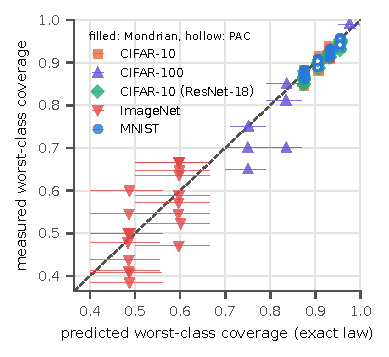
\includegraphics[width=.34\linewidth]{worst_class_theory.pdf}\hfill
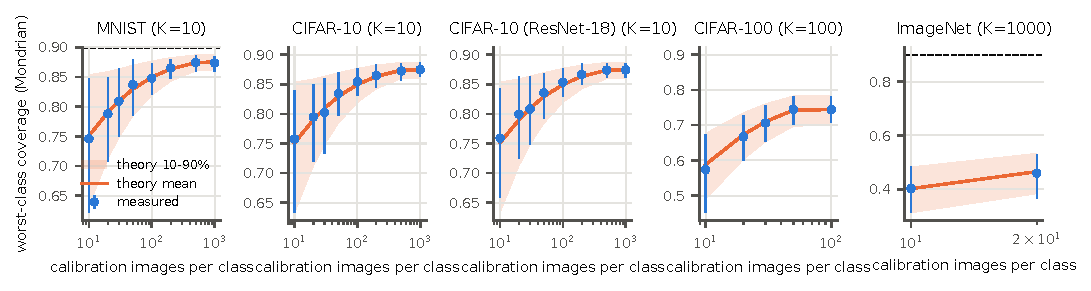
\includegraphics[width=.64\linewidth]{ncal_sweep.pdf}
\caption{Left: measured worst-class coverage against Proposition~\ref{prop:worst} for every run, seed and $\alpha$ (filled: Mondrian, hollow:
Mondrian-PAC; bars: 10--90\% predicted band). Right: worst class vs calibration images per class, from 30 re-splits of $\dcal\cup\dtest$
per point, against the exact law.}
\label{fig:worst}
\end{figure}
\textbf{The worst class is predictable.} Figure~\ref{fig:worst} puts Proposition~\ref{prop:worst} next to experiment. Predicted and
measured Mondrian worst class: MNIST \PredMNISTMond\ vs \MeasMNISTMond\%, CIFAR-10 \PredCTenMond\ vs \MeasCTenMond\%, CIFAR-100
\PredCHunMond\ vs \MeasCHunMond\%, ImageNet \PredINetMond\ vs \MeasINetMond\%. In the re-split sweep, where calibration and test are
exchangeable by construction, the mean measurement is never more than \NsMaxErr\ points from the prediction. On the fixed splits, the
law's probability-integral transform $P(\min\le\text{measured})$ should be uniform over seeds. It is for MNIST (mean \PitMNIST, KS
$p=\KsMNIST$) and for ImageNet (mean \PitINet, KS $p=\KsINet$). On CIFAR-100 it averages \PitCHun\ (Fisher combined $p=\FisherCHun$):
for some classes the official test set is harder than the calibration pool. That is the per-class shift \citet{recht2018cifar}
describe. A coarser $\chi^2$ test on per-class top-1 accuracy (calibration vs test) is weaker there ($p=\ChiPCHun$), yet it fires on
MNIST ($p=\ChiPMNIST$), whose test digits come from different writers, where the worst class is unaffected. For what matters to
coverage, the worst-class law is the sharper diagnostic. With ImageNet's 20 calibration and 20 test images per class, the
``per-class'' method's worst class sits near \MeasINetMond\%. The guarantee holds on average, but it says little about any given
class.

\textbf{High-probability repair and its cost}\label{sec:pac}.
\begin{figure}[t]
\centering
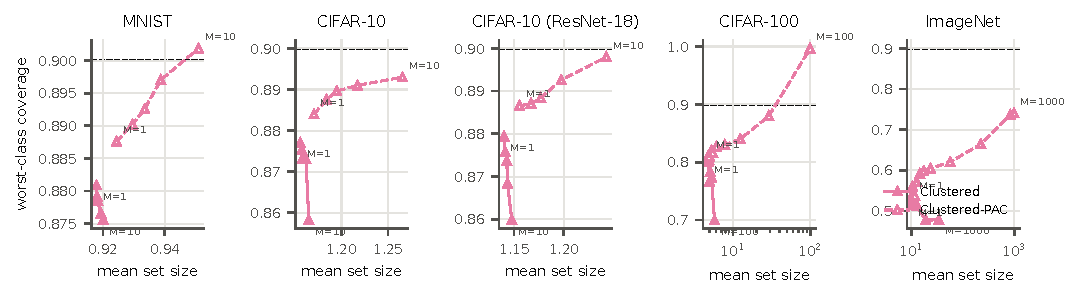
\includegraphics[width=\linewidth]{clusters.pdf}
\caption{Cluster count $M$ from 1 (marginal) to $K$ : mean size vs worst class, without (solid) and with (dashed, hollow) the PAC correction. At $M{=}K$, $k$-means still merges a few classes, so the dashed end point is not exactly Mondrian-PAC (on ImageNet it keeps some finite thresholds).}
\label{fig:clusters}
\end{figure}
Mondrian-PAC lifts the worst class on CIFAR-10 to \WorstCTenMondPAC\% at size \SizeCTenMondPAC. Mondrian alone gives
\WorstCTenMond\% at \SizeCTenMond, and the bootstrap difference is \BsCTenPacVsMondW\ points (95\% CI [\BsCTenPacVsMondWLo,
\BsCTenPacVsMondWHi]). On CIFAR-100 it costs more (\SizeCHunMondPAC\ labels vs \SizeCHunMond). On ImageNet it is infeasible
(Proposition~\ref{prop:pac}) and returns all \SizeINetMondPAC\ labels. Pooling classes fixes this (Figure~\ref{fig:clusters}). On
ImageNet, Clustered-PAC reaches a worst class of \WorstINetClusPAC\% at \SizeINetClusPAC\ labels, above both APS($T$)
(\WorstINetAPST\%, \SizeINetAPST) and Mondrian (\WorstINetMond\%, \SizeINetMond). On CIFAR-100 it reaches \WorstCHunClusPAC\% at
\SizeCHunClusPAC\ labels, where Mondrian-PAC pays \SizeCHunMondPAC\ labels for \WorstCHunMondPAC\%. Only $M=\ClBestMCHun$ clusters
come within a point of Mondrian-PAC's worst class (\ClBestSizeCHun\ labels). On CIFAR-10, $M=\ClBestMCTen$ does so at
\ClBestSizeCTen.

\textbf{Label shift.}
\begin{table}[t]
\centering\small
\caption{Coverage under strong Dirichlet label shift ($\beta=0.1$, mean total-variation shift \LsCTenTv\% on CIFAR-10), mean $\cdot$ worst over draws and seeds.}
\label{tab:ls}
\begin{tabular}{lccccc}
\toprule
& Naive($T$) & APS($T$) & Mondrian & Mondrian-PAC & Weighted (BBSE) \\
\midrule
CIFAR-10 & \LsCTenNaiveMean\,$\cdot$\,\LsCTenNaiveMin & \LsCTenAPSTMean\,$\cdot$\,\LsCTenAPSTMin & \LsCTenMondMean\,$\cdot$\,\LsCTenMondMin & \LsCTenMondPACMean\,$\cdot$\,\LsCTenMondPACMin & \LsCTenBbseMean\,$\cdot$\,\LsCTenBbseMin \\
CIFAR-100 & \LsCHunNaiveMean\,$\cdot$\,\LsCHunNaiveMin & \LsCHunAPSTMean\,$\cdot$\,\LsCHunAPSTMin & \LsCHunMondMean\,$\cdot$\,\LsCHunMondMin & \LsCHunMondPACMean\,$\cdot$\,\LsCHunMondPACMin & \LsCHunBbseMean\,$\cdot$\,\LsCHunBbseMin \\
MNIST & \LsMNISTNaiveMean\,$\cdot$\,\LsMNISTNaiveMin & \LsMNISTAPSTMean\,$\cdot$\,\LsMNISTAPSTMin & \LsMNISTMondMean\,$\cdot$\,\LsMNISTMondMin & \LsMNISTMondPACMean\,$\cdot$\,\LsMNISTMondPACMin & \LsMNISTBbseMean\,$\cdot$\,\LsMNISTBbseMin \\
\bottomrule
\end{tabular}
\end{table}
Table~\ref{tab:ls} shows Corollary~\ref{cor:shift} at work. Under strong label shift, Naive($T$)'s worst draws fall to its worst
class, while the class-wise methods stay near target and Mondrian-PAC stays above it. Label-shift weighted conformal with estimated
BBSE weights \citep{podkopaev2021distribution,lipton2018detecting} also repairs the marginal method, at the cost of estimating $K$
weights.

\textbf{Covariate shift and repairs.}
\begin{figure}[t]
\centering
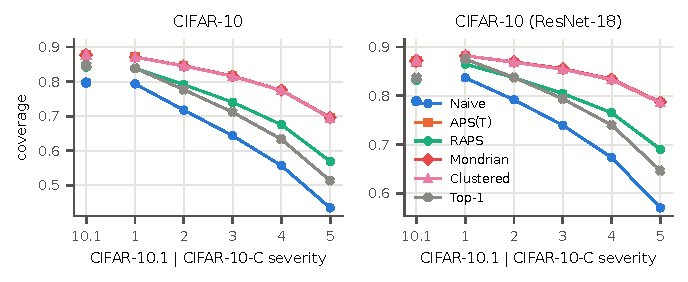
\includegraphics[width=.49\linewidth]{real_shift.pdf}\hfill
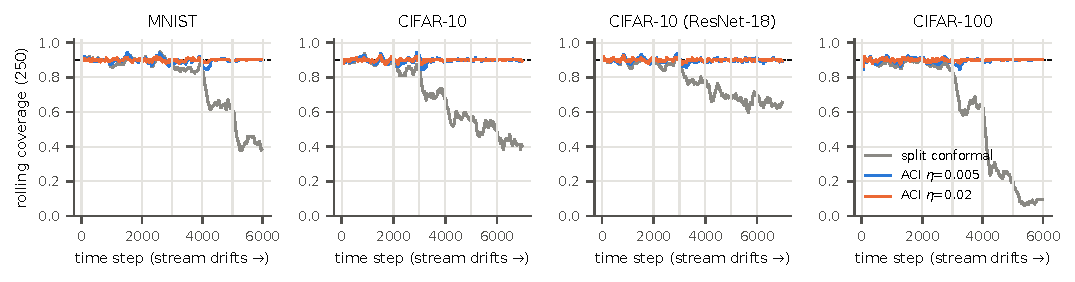
\includegraphics[width=.49\linewidth]{aci.pdf}
\caption{Left: coverage on CIFAR-10.1 (x=0) and CIFAR-10-C severities 1--5 (mean of 15 corruptions). Right: rolling coverage on a stream drifting from clean to severe corruption; split conformal vs ACI.}
\label{fig:shift}
\end{figure}
No guarantee survives a change in $P(X)$. On CIFAR-10.1, a near-copy of the test distribution, APS($T$) covers \TenCTenAPST\% while
accuracy falls to \TenAccCTen\%. At CIFAR-10-C severity 5, coverage averages \CcCTenAPSTSFive\% (Naive: \CcCTenNaiveSFive\%; see
Figure~\ref{fig:shift}). ACI \citep{gibbs2021adaptive} restores long-run coverage on a drifting stream. In the most severe segment of
the CIFAR-10 stream, fixed split conformal covers \AciCTenFixCov\% and ACI \AciCTenAciCov\%, by growing sets from \AciCTenFixSize\ to
\AciCTenAciSize\ labels. Weighted conformal with a feature-space domain classifier \citep{tibshirani2019conformal} lifts coverage on
shifted CIFAR-10 from \WtCovStdCTen\% to \WtCovWCTen\%. But sets grow from \WtSizeStdCTen\ to \WtSizeWCTen\ labels, because \WtInfCTen\%
of images get the full label set. When the classifier separates shifted from clean images almost perfectly, the test point's own
weight exceeds the $\alpha$ budget and the effective calibration size collapses, down to \WtEssMinN\ effective images out of 5,000
\citep{kish1965survey}. On MNIST it barely moves (\WtCovStdMNIST\% to \WtCovWMNIST\%). This is the support-mismatch limit of
covariate-shift conformal.

\textbf{Second architecture and learned score.} With the pretrained ResNet-18 on CIFAR-10 (accuracy \AccCTenR\%), the pattern across
methods does not change (Appendix~\ref{app:tables}). Its worst class under Naive($T$) is \WorstCTenRNaiveT\%, against
\WorstCTenRAPST\% for APS($T$). The learned score reaches size \SizeCTenLearned\ on CIFAR-10, against \SizeCTenNaiveT\ for Naive($T$),
and does not improve the worst class (\WorstCTenLearned\%). Naive is already size-optimal for calibrated probabilities
\citep{sadinle2019least}, so there is little left to learn.

% =====================================================================================================================
\section{Diagnostics}\label{sec:diag}
\textbf{Empty sets.} MNIST at $\alpha=0.1$ returns \EmptyMNISTNaive\% empty sets. Lemma~\ref{lem:empty} predicts at least
\EmptyBoundMnist\%, and the bound held in \EmptyHolds\% of the \EmptyN\ cells where it applies (Appendix Figure~\ref{fig:app2}).
\textbf{Why the distance term helps little.} My first proposal added the Mahalanobis distance of penultimate features to the score,
$s+\gamma\tilde d_M$ \citep{lee2018simple}. It raised CIFAR-10's Naive($T$) worst class by only \BsCTenDistVsNaiveW\ points (CI
[\BsCTenDistVsNaiveWLo, \BsCTenDistVsNaiveWHi]), and $\gamma$ was unstable across seeds. Sets grow by admitting the second-ranked
label. Whether that label is the truth, the softmax decides with AUROC \DdSoftCTen, against \DdDistCTen\ for the distance (CIFAR-100:
\DdSoftCHun\ vs \DdDistCHun). The two are also correlated ($\rho=\DdRhoCTen$). The distance mostly re-weights information the score
already has.
\textbf{Unfamiliar inputs.} Set size is a weak OOD signal. ``Not a singleton'' separates FashionMNIST from MNIST well, but CIFAR-100
from CIFAR-10 poorly (Appendix~\ref{app:figs}).

% =====================================================================================================================
\section{Limitations}
The worst-class law assumes class-wise exchangeability and continuous scores, and it describes class-wise calibration. For marginal
methods the worst class depends on the score, and there is no such law. Clustered-PAC protects clusters, not individual classes. Its
clusters are learned from $\ddes$ (about 10 images per class on ImageNet), so the cluster map is itself noisy. Each run has 3--10
seeds, and the ImageNet seeds re-split one fixed set of outputs from one model. I test synthetic and benchmark corruptions only, not a
real deployment shift. Sweeps over $\gamma$, $M$ and $\eta$ are reported on $\dtest$ as sensitivity checks. The headline numbers use
values fixed on $\ddes$, or defaults stated in advance.

\section{Conclusion}
At a fixed marginal guarantee, the score decides \emph{who} is covered and the grouping decides \emph{which classes} are protected. The
worst class under class-wise calibration can be predicted before deployment: an exact law predicted it in every setting here. The same
law says per-class guarantees at ImageNet scale need thousands of calibration images per class. Sharing corrected thresholds across
clusters of similar classes costs far less: on ImageNet, \SizeINetClusPAC\ labels per set instead of 1{,}000. I recommend reporting
the worst class and the empty-set rate next to marginal coverage, and sizing calibration sets with Corollary~\ref{cor:n}.

\paragraph{Reproducibility and AI-use disclosure.} \texttt{scripts/train\_all.py} trains and caches every run.
\texttt{run\_all.py}, \texttt{sweep.py} and \texttt{research.py} produce every table and figure. \texttt{paper\_numbers.py} writes
every number in this paper as a LaTeX macro, so no result is typed by hand, and 22 unit tests cover the maths. An interactive
companion site re-runs the conformal procedure in the browser. AI assistance (Claude) helped organise the code, build parts of the interactive site and explorers, and edit the report's wording and structure. The experiments, analysis and results are my own.

\bibliographystyle{plainnat}
\bibliography{refs}

% =====================================================================================================================
\appendix
\section{Full tables}\label{app:tables}
\begin{table}[h]
\centering\scriptsize
\caption{All methods at $\alpha=0.1$: MNIST, CIFAR-10 and CIFAR-10 with the pretrained ResNet-18 (mean over seeds).}
\begin{tabular}{lccccccccc}
\toprule
 & \multicolumn{3}{c}{MNIST} & \multicolumn{3}{c}{CIFAR-10} & \multicolumn{3}{c}{CIFAR-10 (ResNet-18)} \\
\cmidrule(lr){2-4} \cmidrule(lr){5-7} \cmidrule(lr){8-10}
Method & Cov. & Size & Worst & Cov. & Size & Worst & Cov. & Size & Worst \\
\midrule
Naive & 0.906 & 0.91 & 0.830 & 0.896 & 0.94 & 0.783 & 0.896 & 0.94 & 0.779 \\
APS & 0.895 & 0.91 & 0.879 & 0.892 & 1.06 & 0.864 & 0.893 & 1.06 & 0.867 \\
RAPS & 0.896 & 0.91 & 0.879 & 0.893 & 1.01 & 0.849 & 0.894 & 1.01 & 0.850 \\
Naive(T) & 0.905 & 0.91 & 0.829 & 0.896 & 0.94 & 0.784 & 0.896 & 0.94 & 0.776 \\
APS(T) & 0.895 & 0.92 & 0.881 & 0.893 & 1.15 & 0.877 & 0.895 & 1.14 & 0.879 \\
Naive(T)+dist & 0.906 & 0.91 & 0.843 & 0.901 & 0.97 & 0.805 & 0.896 & 0.96 & 0.785 \\
APS(T)+dist & 0.896 & 0.92 & 0.882 & 0.893 & 1.15 & 0.877 & 0.896 & 1.14 & 0.880 \\
\addlinespace[2pt]
Margin & 0.906 & 0.91 & 0.830 & 0.895 & 0.94 & 0.783 & 0.896 & 0.94 & 0.777 \\
SAPS & 0.895 & 0.91 & 0.880 & 0.892 & 1.05 & 0.866 & 0.894 & 1.05 & 0.870 \\
Learned & 0.905 & 0.91 & 0.820 & 0.896 & 0.94 & 0.771 & 0.893 & 0.94 & 0.740 \\
\addlinespace[2pt]
Mondrian & 0.897 & 0.92 & 0.875 & 0.894 & 1.16 & 0.864 & 0.896 & 1.15 & 0.860 \\
Mondrian-PAC & 0.923 & 0.95 & 0.902 & 0.923 & 1.26 & 0.896 & 0.924 & 1.24 & 0.898 \\
Clustered & 0.896 & 0.92 & 0.879 & 0.893 & 1.15 & 0.872 & 0.896 & 1.14 & 0.874 \\
Clustered-PAC & 0.909 & 0.93 & 0.893 & 0.905 & 1.19 & 0.887 & 0.907 & 1.18 & 0.888 \\
Top-1 & 0.991 & 1.00 & 0.982 & 0.923 & 1.00 & 0.839 & 0.924 & 1.00 & 0.836 \\
\bottomrule
\end{tabular}

\end{table}
\begin{table}[h]
\centering\scriptsize
\caption{All methods at $\alpha=0.1$: CIFAR-100 and ImageNet (size $\pm$ std over seeds).}
\begin{tabular}{lcccccc}
\toprule
 & \multicolumn{3}{c}{CIFAR-100} & \multicolumn{3}{c}{ImageNet} \\
\cmidrule(lr){2-4} \cmidrule(lr){5-7}
Method & Cov. & Size & Worst & Cov. & Size & Worst \\
\midrule
Naive & 0.897 & 2.54\,{\scriptsize$\pm$0.09} & 0.750 & 0.899 & 1.76\,{\scriptsize$\pm$0.04} & 0.390 \\
APS & 0.895 & 3.81\,{\scriptsize$\pm$0.13} & 0.777 & 0.899 & 6.27\,{\scriptsize$\pm$0.21} & 0.500 \\
RAPS & 0.894 & 2.79\,{\scriptsize$\pm$0.07} & 0.740 & 0.900 & 1.92\,{\scriptsize$\pm$0.06} & 0.389 \\
Naive(T) & 0.896 & 2.47\,{\scriptsize$\pm$0.08} & 0.730 & 0.899 & 1.75\,{\scriptsize$\pm$0.04} & 0.379 \\
APS(T) & 0.893 & 4.78\,{\scriptsize$\pm$0.23} & 0.807 & 0.900 & 10.27\,{\scriptsize$\pm$0.37} & 0.529 \\
Naive(T)+dist & 0.896 & 2.47\,{\scriptsize$\pm$0.09} & 0.733 & -- & -- & -- \\
APS(T)+dist & 0.893 & 5.02\,{\scriptsize$\pm$0.18} & 0.760 & -- & -- & -- \\
\addlinespace[2pt]
Margin & 0.894 & 19.14\,{\scriptsize$\pm$0.88} & 0.753 & 0.901 & 99.90\,{\scriptsize$\pm$4.66} & 0.420 \\
SAPS & 0.897 & 2.76\,{\scriptsize$\pm$0.10} & 0.727 & 0.899 & 1.98\,{\scriptsize$\pm$0.02} & 0.396 \\
Learned & 0.896 & 2.51\,{\scriptsize$\pm$0.09} & 0.723 & 0.899 & 1.76\,{\scriptsize$\pm$0.03} & 0.392 \\
\addlinespace[2pt]
Mondrian & 0.901 & 5.79\,{\scriptsize$\pm$0.40} & 0.700 & 0.923 & 34.96\,{\scriptsize$\pm$2.21} & 0.477 \\
Mondrian-PAC & 1.000 & 99.41\,{\scriptsize$\pm$1.02} & 0.997 & 1.000 & 1000\,{\scriptsize$\pm$0.00} & 1.000 \\
Clustered & 0.893 & 4.87\,{\scriptsize$\pm$0.24} & 0.803 & 0.901 & 10.74\,{\scriptsize$\pm$0.34} & 0.529 \\
Clustered-PAC & 0.920 & 6.14\,{\scriptsize$\pm$0.29} & 0.827 & 0.929 & 17.18\,{\scriptsize$\pm$1.09} & 0.607 \\
Top-1 & 0.710 & 1.00\,{\scriptsize$\pm$0.00} & 0.430 & 0.784 & 1.00\,{\scriptsize$\pm$0.00} & 0.133 \\
\bottomrule
\end{tabular}

\end{table}

\section{Additional figures}\label{app:figs}
\begin{figure}[h]
\centering
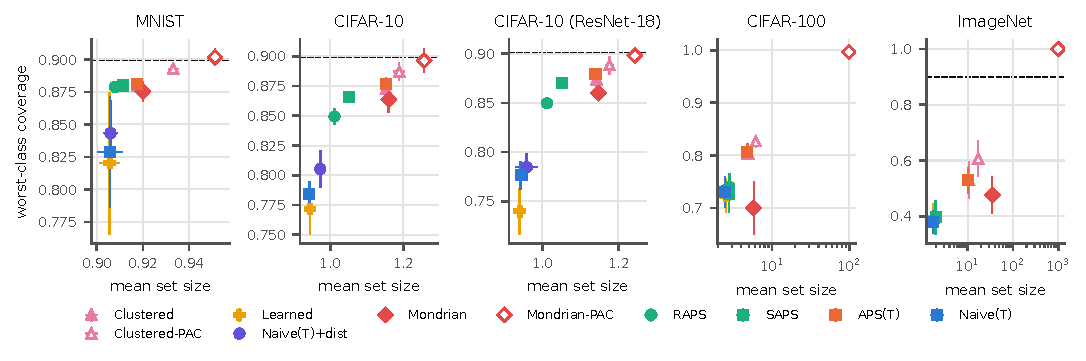
\includegraphics[width=\linewidth]{frontier.pdf}\\[2pt]
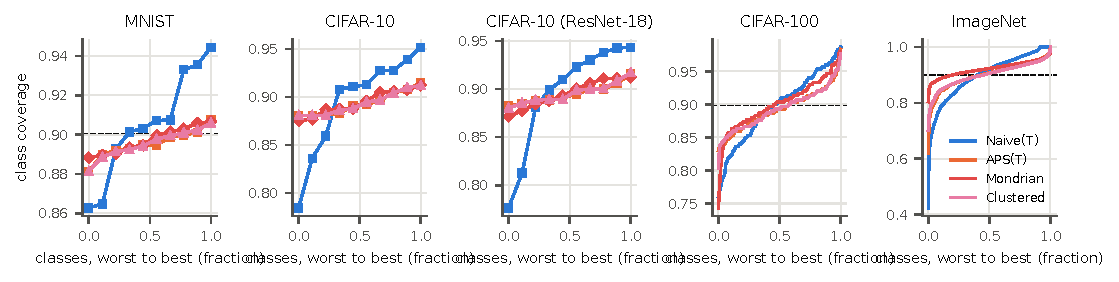
\includegraphics[width=\linewidth]{class_coverage.pdf}
\caption{Top: efficiency frontier (mean size vs worst class). Bottom: per-class coverage sorted from worst to best.}
\label{fig:app1}
\end{figure}
\begin{figure}[h]
\centering
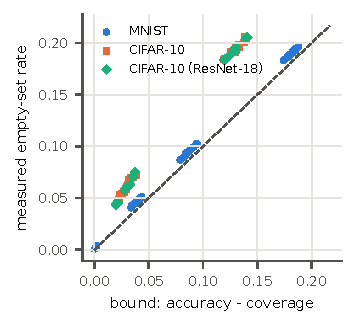
\includegraphics[width=.33\linewidth]{empty_bound.pdf}\hfill
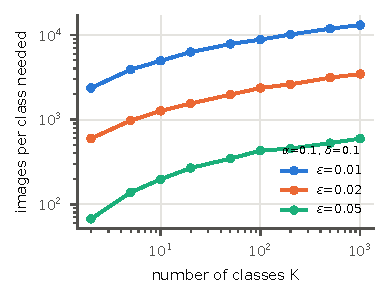
\includegraphics[width=.33\linewidth]{n_needed.pdf}\hfill
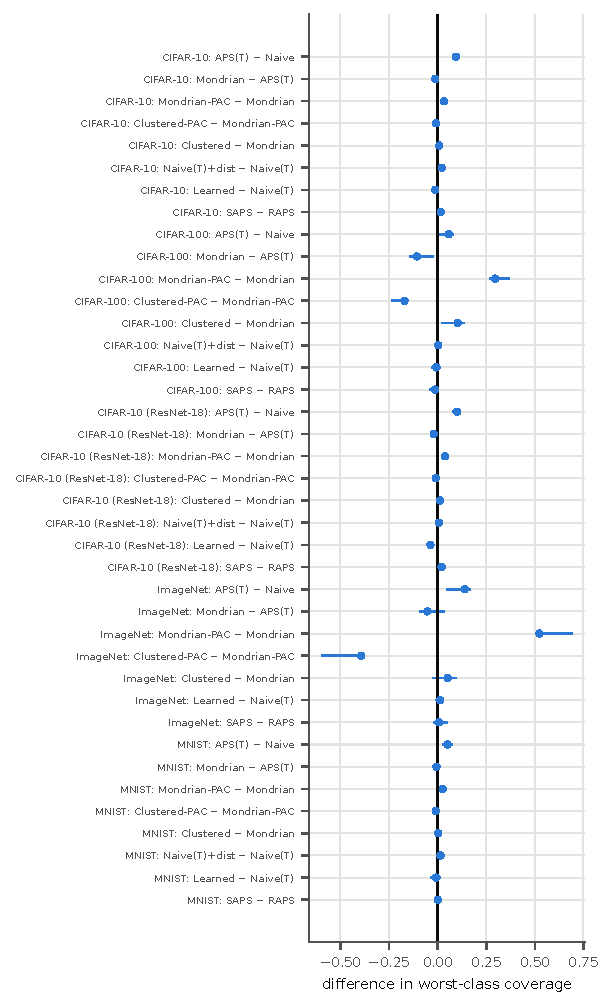
\includegraphics[width=.32\linewidth]{bootstrap_worst.pdf}
\caption{Left: empty-set rate vs Lemma~\ref{lem:empty}. Middle: Corollary~\ref{cor:n}. Right: hierarchical-bootstrap 95\% intervals for worst-class differences.}
\label{fig:app2}
\end{figure}
\begin{figure}[h]
\centering
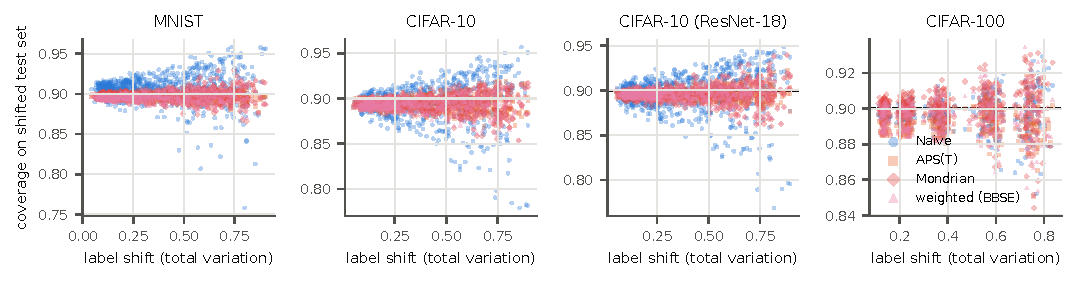
\includegraphics[width=\linewidth]{label_shift.pdf}\\[2pt]
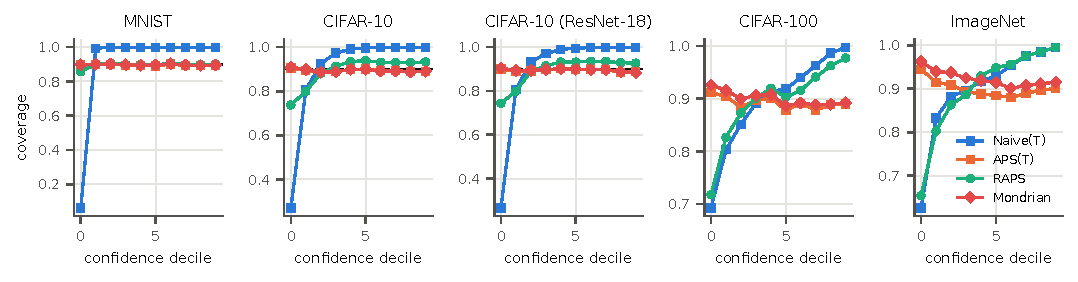
\includegraphics[width=\linewidth]{decile_coverage.pdf}\\[2pt]
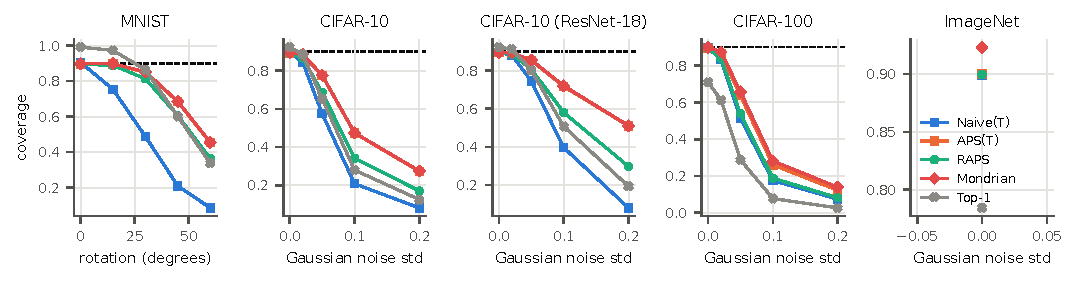
\includegraphics[width=\linewidth]{shift.pdf}
\caption{Top: coverage vs size of a Dirichlet label shift. Middle: coverage by confidence decile. Bottom: synthetic covariate shift.}
\end{figure}
\begin{figure}[h]
\centering
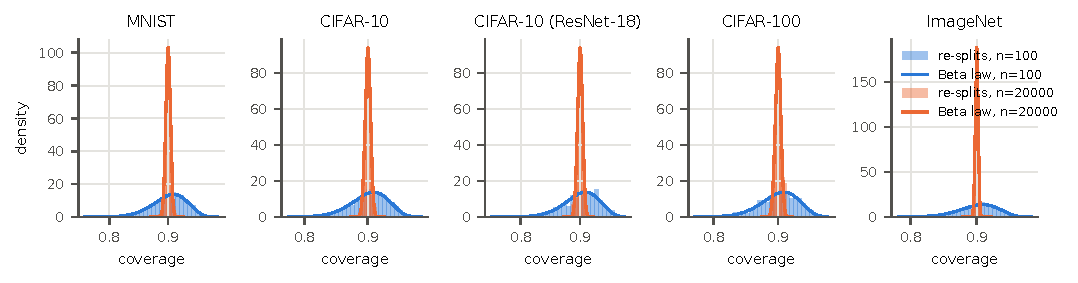
\includegraphics[width=\linewidth]{resplit.pdf}\\[2pt]
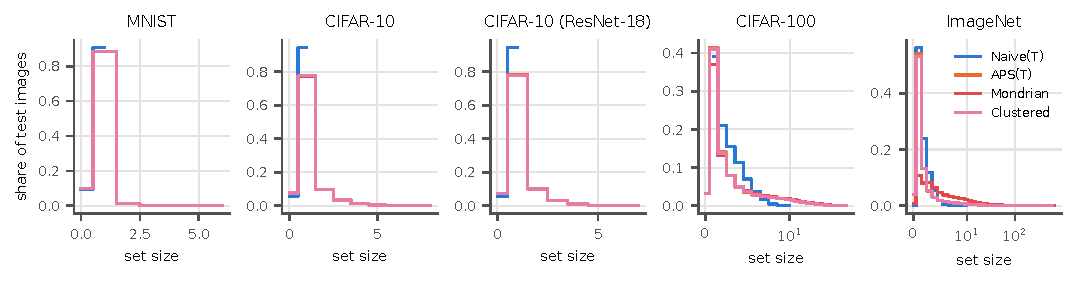
\includegraphics[width=\linewidth]{set_sizes.pdf}\\[2pt]
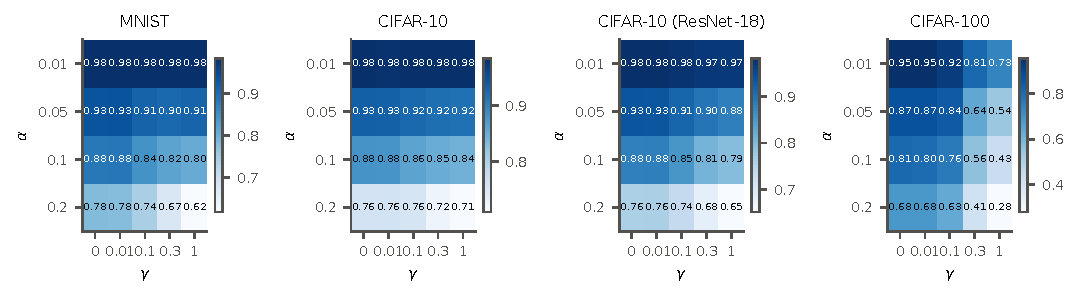
\includegraphics[width=\linewidth]{sweep_min_cov.pdf}
\caption{Top: coverage over random re-splits vs the marginal Beta law. Middle: set-size distributions. Bottom: worst class over the $\alpha\times\gamma$ grid for APS($T$)+distance.}
\end{figure}

\section{Implementation details}
LeNet (2 conv + 2 FC, Adam $10^{-3}$, 10 epochs); SmallResNet (3 stages $\times$ 2 basic blocks, SGD+Nesterov, OneCycle to 0.1, weight decay
$5\cdot10^{-4}$, 30 epochs, flip+crop); ResNet-18 (torchvision ImageNet weights, inputs upsampled to $64\times64$, OneCycle to 0.02, 12 epochs).
Early stopping on $\ddes$ NLL. $T$ by LBFGS on $\ddes$ NLL. RAPS $(\lambda,k_\text{reg})\in\{0.01,0.05,0.1\}\times\{1,2,5\}$ and SAPS
$\lambda\in\{0.01,0.05,0.1,0.2,0.4\}$ minimise $\ddes$ mean size by two-fold calibration on $\ddes$; $\gamma\in\{0,0.01,0.1,0.3,1\}$ maximises
$\ddes$ worst class subject to size $\le1.1\times$ the $\gamma{=}0$ size. Learned score: residual MLP ($K\!\to\!64\!\to\!K$, zero-initialised
output) on $\log p_T$, Adam $10^{-3}$, 400 steps of batch 1000 on half of $\ddes$, smooth size loss $\max(0,\sum_y\sigma((\hat q-s_y)/0.1)-1)$
plus cross-entropy, early-stopped on the other half by exact size. Clusters: weighted $k$-means ($\sqrt{n_c}$ weights, $k$-means++ init)
on the 0.5--0.9 quantiles of each class's $\ddes$ APS($T$) scores; classes with $<5$ points use the marginal threshold. FSC: 10 $k$-means
clusters of $D_\text{train}$ features. Domain classifier: $\ell_2$ logistic regression on standardised features ($\ddes$ vs half of the
shifted set), weights clipped at 100. ACI: $\eta\in\{0,0.005,0.02\}$ on APS($T$).
\end{document}
